\documentclass[a4paper,twoside,openright,makeidx,12pt]{book}
%\usepackage{draftcopy}
%$Id: macro.tex,v 1.10 2004/12/08 13:38:58 acary Exp $


%\usepackage{a4wide}
\textheight 25cm
\textwidth 16.5cm
\topmargin -1cm
%\evensidemargin 0cm
\oddsidemargin 0cm
\evensidemargin0cm
\usepackage{layout}


\usepackage{amsmath}
\usepackage{amssymb}
\usepackage{minitoc}
%\usepackage{glosstex}
\usepackage{colortbl}
\usepackage{hhline}
\usepackage{longtable}

%\usepackage{glosstex}
%\def\glossaryname{Glossary of Notation}
\def\listacronymname{Acronyms}

\usepackage[outerbars]{changebar}\setcounter{changebargrey}{20}
%\glxitemorderdefault{acr}{l}

%\usepackage{color}
\usepackage{graphicx,epsfig}
\graphicspath{{figure/}}
\usepackage[T1]{fontenc}
\usepackage{rotating}

%\usepackage{algorithmic}
%\usepackage{algorithm}
\usepackage{ntheorem}
\usepackage{natbib}


%\renewcommand{\baselinestretch}{2.0}
\setcounter{tocdepth}{2}     % Dans la table des matieres
\setcounter{secnumdepth}{3}  % Avec un numero.



\newtheorem{definition}{Definition}
\newtheorem{lemma}{Lemma}
\newtheorem{claim}{Claim}
\newtheorem{remark}{Remark}
\newtheorem{assumption}{Assumption}
\newtheorem{example}{Example}
\newtheorem{conjecture}{Conjecture}
\newtheorem{corollary}{Corollary}
\newtheorem{OP}{OP}
\newtheorem{problem}{Problem}
\newtheorem{theorem}{Theorem}


\newcommand{\CC}{\mbox{\rm $~\vrule height6.6pt width0.5pt depth0.25pt\!\!$C}}
\newcommand{\ZZ}{\mbox{\rm \lower0.3pt\hbox{$\angle\!\!\!$}Z}}
\newcommand{\RR}{\mbox{\rm $I\!\!R$}}
\newcommand{\NN}{\mbox{\rm $I\!\!N$}}

\newcommand{\Mnn}{\mathcal M^{n\times n}}
\newcommand{\Mnp}[2]{\ensuremath{\mathcal M^{#1\times #2}}}



\newcommand{\Frac}[2]{\displaystyle \frac{#1}{#2}}

\newcommand{\DP}[2]{\displaystyle \frac{\partial {#1}}{\partial {#2}}}

% c++ variables writting
\newcommand{\varcpp}[1]{\textit{#1}}
% itemize
\newcommand{\bei}{\begin{itemize}}
\newcommand{\ei}{\end{itemize}}

\newcommand{\ie}{i.e.}
\newcommand{\eg}{e.g.}
\newcommand{\cf}{c.f.}
\newcommand{\putidx}[1]{\index{#1}\textit{#1}}

\def\Er{{\rm I\! R}}
\def\En{{\rm I\! N}} 
\def\Ec{{\rm I\! C}}
 
\def\zc{\hat{z}}
\def\wc{\hat{w}}

\font\tete=cmr8 at 8 pt
\font\titre= cmr12 at 20 pt 
\font\titregras=cmbx12 at 20 pt

%----------------------------------------------------------------------
%                  Modification des subsubsections
%----------------------------------------------------------------------
\makeatletter
\renewcommand\thesubsubsection{\thesubsection.\@alph\c@subsubsection}
\makeatother

%----------------------------------------------------------------------
%             Redaction note environnement
%----------------------------------------------------------------------
\makeatletter
\theoremheaderfont{\scshape}
\theoremstyle{marginbreak}
\theorembodyfont{\upshape}
%\newtheorem{rque}{\bf Remarque}[chapter]
%\newtheorem{rque1}{\bf \fsc{Remarque}}[chapter] !!! \fsc est une commande french
\newtheorem{ndr1}{\textbf{\textsc{Redaction note}}}[section]

\newenvironment{ndr}%
{%
\tt
%\centerline{---oOo---}
\noindent\begin{ndr1}%
}%
{%
\begin{flushright}%
%\vspace{-1.5em}\ding{111}
\end{flushright}%
\end{ndr1}%
%\centerline{---oOo---}
}

\makeatother

%----------------------------------------------------------------------
%             Redaction note environnement V.ACARY
%----------------------------------------------------------------------
\makeatletter
\theoremheaderfont{\scshape}
\theoremstyle{marginbreak}
\theorembodyfont{\upshape}
%\newtheorem{rque}{\bf Remarque}[chapter]
%\newtheorem{rque1}{\bf \fsc{Remarque}}[chapter] !!! \fsc est une commande french
\newtheorem{ndr1va}{\textbf{\textsc{Redaction note V. ACARY}}}[section]

\newenvironment{ndrva}%
{%
\tt
%\centerline{---oOo---}
\noindent\begin{ndr1va}%
}%
{%
\begin{flushright}%
%\vspace{-1.5em}\ding{111}
\end{flushright}%
\end{ndr1va}%
%\centerline{---oOo---}
}

\makeatother
%----------------------------------------------------------------------
%             Redaction note environnement V.ACARY
%----------------------------------------------------------------------
\makeatletter
\theoremheaderfont{\scshape}
\theoremstyle{marginbreak}
\theorembodyfont{\upshape}
%\newtheorem{rque}{\bf Remarque}[chapter]
%\newtheorem{rque1}{\bf \fsc{Remarque}}[chapter] !!! \fsc est une commande french
\newtheorem{ndr1fp}{\textbf{\textsc{Redaction note F. PERIGNON}}}[section]

\newenvironment{ndrfp}%
{%
\tt
%\centerline{---oOo---}
\noindent\begin{ndr1fp}%
}%
{%
\begin{flushright}%
%\vspace{-1.5em}\ding{111}
\end{flushright}%
\end{ndr1fp}%
%\centerline{---oOo---}
}

\makeatother
%----------------------------------------------------------------------
%                  Chapter head enviroment
%----------------------------------------------------------------------
\newenvironment{chapter_head}
{%
\begin{center}%
-------------------- oOo --------------------\\%
\ \\%
\begin{minipage}[]{14cm}%
\noindent\normalsize\advance\baselineskip-1pt %
}%
{%
\par\end{minipage}%
\ \\%
\ \\%
-------------------- oOo --------------------
\end{center}%
\vspace*{\stretch{1}}%
\clearpage%
\thispagestyle{empty}%
\vspace*{\stretch{1}}%
\minitoc%
\vspace*{\stretch{2}}%
\clearpage%
}

%%% Local Variables: 
%%% mode: latex
%%% TeX-master: "report"
%%% End: 


\glxitemorderdefault{acr}{s}

\includeonly{}
\usepackage{fancyheadings} 
\usepackage{verbatim} 

% package pour les images des use cases
%\usepackage[dvips]{graphicx}

\pagestyle{fancy} 
\renewcommand{\chaptermark}[1]% 
{\markboth{{Chap-- \thechapter.\ #1}}{}} 
\renewcommand{\sectionmark}[1]% 
{\markright{{\thesection.\ #1}}} 
\setlength{\headrulewidth}{0.5pt} 
\setlength{\footrulewidth}{0.5pt} 
\newcommand{\helv}{% 
\fontfamily{phv}\fontseries{b}\fontsize{9}{11}\selectfont} 
\lhead[\helv \thepage]{\helv \rightmark} 
\rhead[\helv \leftmark]{\helv \thepage} 
\cfoot{\acs{um} -- \today}

\makeindex

\begin{document}
\pagestyle{empty}
\renewcommand{\arraystretch}{1.8}

%%%%%%%%%%%%%%%%%%%%%%%%%%%%%%%%%%%%%%%%%%%%%%%%%%%%%%%%%%%%%%%%%%%%%%%%%%%%%%%%%%%%%%%%%%%%%%%%%%%%%%%%%
%\documentclass[titlepage, 12pt]{report}

%\usepackage[dvips]{graphicx}
%\usepackage{graphics}
%\usepackage{amssymb}
%\usepackage{latexsym}


%\begin{document}

\thispagestyle{empty}

\begin{center}

\includegraphics[height=23mm, width=77mm]{figure/siconos.eps}\\
\textsf{Siconos Project}\\[6cm]
\end{center}

\begin{center}
\huge
\textsf{\textbf{\textit{Software User Manual}}}\\[2.5cm]
\end{center}

\large
\begin{center}
\textsf{\textbf{Version :} 0.1}\\
\textsf{\textbf{Status :}  In progress}\\
\textsf{\textbf{Date : } November 25, 2004}\\
\textsf{\textbf{Document Code :} NUMERICS/SUM}\\[5cm]

\end{center}

\normalsize

\begin{flushright}

\includegraphics[scale=0.3]{figure/Logo-INRIA.eps}
\end{flushright}

\clearpage




%\maketitle

%-----------------------------------------------------------------------------%

\normalsize

\begin{center}
  \textsf{\Large Identification}
\end{center}

\noindent\begin{tabular}{|p{0.3\textwidth}|p{0.7\textwidth}|}
\hline
Document Title : & \textsf{Software Specification Document} \\
Document Code :  & \textsf{NUMERICS/SUM} \\
\hline
\end{tabular}
\textsf{ }\\


\begin{center}
  \textsf{\Large About the document and its author(s)}
\end{center}

\noindent\begin{tabular}{|p{0.3\textwidth}|p{0.7\textwidth}|}
\hline
Nature :& \textsf{This document defines the User Manual for Numerics}\\
Language :& \textsf{English}\\
Author(s) :& \textsf{Fr�d�ric DUBOIS, Jean-Michel BARBIER}\\
Possible remarks :& \textsf{}\\
References : & \\
\hline
\end{tabular}

\textsf{ }\\

%\newpage

% cartridge current version
\renewcommand{\arraystretch}{1.0}
\begin{center}
  \textsf{\Large Current Version}
\end{center}
\begin{tabular}{|p{0.3\textwidth}|p{0.7\textwidth}|}
\hline
Date : &\textsf{November 25, 2004}\\
Current version number : &\textsf{0.1}\\ 
Status :&$\bigotimes$ in progress \\
& $\bigcirc$ validated\\
\textit{ }& \hspace{0.5cm} Approved by :\\
\hline
\end{tabular}


\textsf{ }\\
\begin{center}
\textbf{Copyright Notice \copyright}\\
This document may not be reproduced (even partially) or communicated to third parties without the written authorisation of LMGC.
\end{center}
\renewcommand{\arraystretch}{1.8}


% log of changes  
\pagebreak
\begin{center}
  \textsf{\Large About the document developing process}
\end{center}
\begin{tabular}{|p{0.3\textwidth}|p{0.7\textwidth}|}
\hline
Date of first issue : &\textsf{November 25, 2004}\\
Current version number : &\textsf{0.1}\\ 
Validated by :& \textsf{}\\
\hline
Document change record since last version : &\textsf{First issue} \\
\hline

\end{tabular}

%\end{document}

%%%%%%%%%%%%%%%%%%%%%%%%%%%%%%%%%%%%%%%%%%%%%%%%%%%%%%%%%%%%%%%%%%%%%%%%%%%%%%%%%%%%%%%%%%%%%%%%%%%%%%%%%


\tableofcontents
\cleardoublepage

\pagestyle{fancy}
%---------------------------------------------------------------------%
\clearpage
\pagenumbering{arabic}
%---------------------------------------------------------------------%


%---------------------------------------------------------------------%
\chapter{Introduction}
\label{Sec:UM-Intoduction}
\section{Purpose of this document}
\label{Sec:SUM-Purpose-Scope}
The purpose of the Software User Manual is to ...

%---------------------------------------------------------------------%

%---------------------------------------------------------------------%
\chapter{Overview}
\label{Sec:UM-Overview}
The \ac{siconos} platform is dedicated to the modelling and simulation of \ac{nsds}. For modelling part, several canonical model for \ac{nsds}, relations and non-smooth laws can be used. For the simulation part, robust time integration method (time stepping, event driven) of the dynamics and numerical solvers for non smooth laws can be used.

The \ac{siconos} platform can be used as a library.

The numerical routine for computation is provide by plugin. Each user can develop his own plugin and use it

The \ac{siconos} platform can take as input file an \ac{xml} file which describe the system. The platform can formalise the input file into canonical model, and analyse the coherence of the data. It can make an \ac{xml} file in order to save the state of the system during and / or after the simulation.

Expert user can modify the platform and add some functionality, because this platform is open source. Some documents will help developers (\ac{ddd}, \ac{esd}, \ac{anp}, ...)

\textbf{
In this version of \ac{siconos}, for driving a simulation, the user have to write a command file (in C++). This file creates dynamical systems, interactions, \dots run the simulation and collect informations.
}

%---------------------------------------------------------------------%

%---------------------------------------------------------------------%
\chapter{Platform Architecture}
\label{Sec:UM-Archi}
Two deliverables can be distributed, corresponding to the two main uses of the platform~: a basic one for end-users, with only binaries, and a complete one with source files, to allow users to develop news functionalities for the software.
Here we describe the architecture of the distribution for end users. Developers can refer to the \ac{ddd} for complete architecture.

\section{Files and directories}
The software \textit{siconos} will be a set of C++ libraries driven by a main program. This kind of libraries are named in the following as "internal libraries" (i.e. libraries developed in \ac{siconos}, in opposition to the "external libraries" which are for example libXML2 or Lapack++). \\

In this distribution, the root directory is named \textit{SICONOS/}. It contains the following sub-directories and files~: 
\begin{itemize}

\item  \textit{bin/} : contains binaries of the platform.

\item \textit{include/} : contains header files of internal libraries.

\item \textit{lib/} : contains the libraries of the platform.

\item \textit{share/} : contains some configuration files, necessary ton run a simulation with the platform : \acs{xml} schema, ...

\end{itemize}


%\section{User data}
%Each system which is simulated by the platform must have a particular workspace, which is a directory. The path of the directory should be given by the user. By default, simulations files (\ac{xml} files and vector / matrix data files) are placed in the \textit{samples} directory of the platform.

%---------------------------------------------------------------------%

%---------------------------------------------------------------------%
\chapter{Instructions}
\label{Sec:UM-Intructions}
\section{Installation of the platform}

\subsection{get sources of the platform}

You have to download the sources from our SCN server (see http://gforge.inria.fr/projects/siconos for instructions).

\subsection{External libraries}

The platform needs some external libraries to compile:
\begin{itemize}

\item Siconos Numerics

\item libxml2

\item lapack++

\item lapack and blas

\item nana
\end{itemize}

To know the required versions and where these libraries are available on the web, please look at the siconos gforge site (http://gforge.inria.fr/projects/siconos).


\subsection{Generation of configure script}

The platform version of SVN is a developer version and is not ready to be installed. You have to run a script to generate configuration script.
This script is situated in Kernel directory.
\begin{verbatim}
% ./reconf.sh
\end{verbatim}


\subsection{Run configure script}
By default, the platform is installed in /usr/local (you must be logged as root to be allowed to write some files in this directory).
\begin{verbatim}
% ./configure
\end{verbatim} 

To set another installation directory, use --prefix=path flag. for example :
\begin{verbatim}
% ./configure --prefix=/home/User/Siconos
\end{verbatim} 

There may be some parameters to set; to know them, run 
\begin{verbatim}
% configure --help 
\end{verbatim}

If an external library is not installed in /usr or /usr/local, you have to give its path to configure script by the flag : --with-local[\textit{library name}]=[\textit{path of this library}].

For example : 
\begin{verbatim}
% ./configure --with-localnana=/home/User/nana-2.5
\end{verbatim}

\textit{\textbf{Nota:} you have only to run configure script once, you can specify several flags together. }

\subsection{compiling the platform}
\begin{verbatim}
% make
\end{verbatim}
This command compiles the platform and creates libraries.

\subsection{Installing the platform}
\begin{verbatim}
% make install
\end{verbatim}
this command installs the platform in /usr/local by default, or in the directory specified during configure running.




\section{Launch the platform}\label{run}
First of all, you have to set a \verb+SICONOSPATH+ environment variable to the complete path of the siconos install directory\footnote{for example "\$HOME/SICONOS" }. 
The input files are :
\begin{itemize}
\item a command file in C++(like \textit{command.cpp}) which lead the execution\footnote{too see an example of command file report to Annexe A}~;
\item an \ac{xml} file which describes your system\footnote{it is optional. Anyway, you can put it in another directory}.
\item all the plugin you want to use in a C file (like \textit{myPlugin.c}). Its name must finish by �Plugin.c�
\end{itemize}
Run the command (we assume you are in the directory containing your command file): 
\begin{verbatim}
%  siconos yourCommandFile.cpp
\end{verbatim}
This will compile your plugins (if there are), your command file and link it to the platform.
In your command file, you can for example create a model using an \ac{xml} file place in the \textit{sample} directory.\\

Remark :
\begin{enumerate}
\item The siconos executable are placed in the same directory of your command file. If you want to run this file without the siconos script, you have to specify in environment variable \verb+LD_LIBRARY_PATH+ the paths of the shared libraries needed by the platform : plugins, lib directory of your siconos installation. \\
\item If you want to use a plugin which is not in the directory \textit{sample} or in the directory \textit{src/plugin}, you must modify the \verb+LD_LIBRARY_PATH+ environment variable. It tell where to find libraries and plugins, so don't forget to add the path to this plugin in this environment variable (see \ref{plugin}) Note that this plugin will NOT be compiled automatically by the siconos script.
\end{enumerate}


\section{Modify the platform}
If you have the source files of the platform, you can modify them.
After that, you must re-compile the platform with~:
\begin{verbatim}
%  make
\end{verbatim}

\section{Test the platform} 
If you modify the platform, you should run test to validate your modification. Do (cppUnit must be installed):
\begin{verbatim}
%  make check
\end{verbatim}

This will launch a test suite with CppUnit.
If you add a class or a function, don't forget to make a test class.

All commands can be launch on the root directory (all, clean, check) or in a specified directory.

\section{Make a plugin}\label{plugin}


To make a plugin, create a file \textit{MyPlugin.c} and declare your functions with \verb+extern "C"+. The name of the plugin file must end by \textit{Plugin.c} : myPlugin.c, electronical\_Plugin.c are correct, error\_plugin.c or badName.c are not. If the name of your plugin does not respect this rule, the siconos script will not automatically compile and add it to \verb+LD_LIBRARY_PATH+ before running. Example for a vector field function~:
\begin{verbatim}
extern "C" void vectorField(int sizeOfX, double time, double& xPtr, double& xdotPtr)
{
    /* input parameter : sizeOfX (size of the vector X); 
     *                     time ; xPtr (pointer to X vector); 
     * output parameter : xdotPtr (pointer to Xdot vector)
     */

/*.....*/
}
\end{verbatim}
You must respect the parameter order for each function you declare. You can look at the \textit{BasicPlugin.c} file in \textit{src/plugin} directory to see examples.
If you do not use the siconos script to compile the plugin :
To compile the plugin, do (we assume tou have g++ 3.*.* and your OS is Linux):
\begin{verbatim}
%  g++ -c myPlugin.c
%  g++ -shared  myPlugin.o -o myPlugin.so
\end{verbatim}
The plugin \textit{myPlugin.so} is now created.
To use it, you have to precise its name and the function name in the \ac{xml} file (see xml part).
You can add the complete plugin path to the \verb+LD_LIBRARY_PATH+ environment variable. If you don't do this, you have to precise it in the \ac{siconos} \ac{xml} file.



%---------------------------------------------------------------------%

%---------------------------------------------------------------------%
\chapter{Input/Output Siconos XML files}
\label{Sec:UM-XML}
This chapter allows to know how to understand and create Input/Output Siconos \ac{xml} files.

\section{General type syntax}
Certain Siconos \ac{xml} tags have complex types, we are going to see in this section.

\subsection{Plugin type}
Some tags are defined with a plugin type : it allows you to indicate functions you want to use in order to compute values.

The syntax to indicate a plugin is always the same : first the name of the library (without it extension), then the function
name ; separated with a double point.\\
For example : 'libraryNameYouWantToUse\textbf{:}theLibraryFunctionYouWantToUse'\\

The plugin tags have no content ; only an attribute to indicate the plugin to use, and which the name is \textit{plugin}.\\

For example : <TagPlugin \textbf{plugin}='myLib:myFunction'/>\\


\subsection{Matrix and Vector syntax}

Several Siconos tags are vector double or matrix double type. In a Siconos \ac{xml} file, it exists several ways to represent a vector or a matrix. 
 
A computed representation is even possible (using plugin).\\


\subsubsection{Vector representation}

In this section we consider that \textit{myVector} is a \ac{xml} tag with vector type.\\

\begin{itemize}

\item \textbf{Give directly a vector double values}\\

If you want to give directly the values of a vector in a Siconos \ac{xml} file, you have just to precise double values in the content of the concerned
 \ac{xml} tag, and indicate the vector size (positive integer value) in an attribute whose name is \textit{vectorSize}.\\


For example : \\

<myVector \textbf{vectorSize}='4'>\\
\verb+  45.554 5465.5 99+ \\
\verb+			54 +\\
</myVector>\\


Note that vector values must be separated with spaces, tabs, or broken lines.\\


\item \textbf{Precise a file who contents vector values}\\

You can also set a vector with a vector represented in a ASCII file.

To precise a simple vector in a file, just write the 1 number (this first number represents the number of sub vector ; here one), then the size of your vector, and at last it double values (different values can/must be separated with spaces, tabs or
broken lines). \\

For example : \\
\textit{myVectorFile.dat}
\verb+1	5 +\\
\verb+1.2 21. 5 2e5 4.5454+\\


Therefore, you can use your file and precise it in a \ac{xml} tag ; just indicate in a \textit{vectorFile} attribute of the vector tag the name of the concerned file :\\

<myVector \textbf{vectorFile}='myVectorFile.dat'/>\\


\item \textbf{Precise a plugin who computes the vector value}\\

A last solution consists to give a plugin which will compute the value of the vector. Just indicate the plugin in a \textit{vectorPlugin} attribute : \\

<myVector \textbf{vectorPlugin}='myLib:myFunction'/>\\

\end{itemize}

\subsubsection{Matrix representation}

In this section we consider that \textit{myMatrix} is a \ac{xml} tag with matrix type.\\

\begin{itemize}

\item \textbf{Give directly a matrix double values}\\

If you want to give directly the values of a matrix in a Siconos \ac{xml} file, first you have to indicate the matrix size (positive integer values) in the following attributes : \textit{matrixRowSize} (the row size of the matrix) and
 \textit{matrixColSize} (the column size of the matrix). Then, each row double values of the matrix have to be contained in a \textit{row} tag. \\


For example : \\

<myMatrix \textbf{matrixRowSize}='3' \textbf{matrixColSize}='2'>  \\
\verb+	<row>45.554 5.08 </row>+\\
\verb+	<row>95.4	-54 </row>+\\
\verb+	<row>6e-4	4e-5 </row>+\\
</myMatrix>\\


Note that, like vector type, double values in row matrix content must be separated with spaces, tabs, or break lines.\\


\item \textbf{Precise a file who contents matrix values}\\

You can also set a matrix with a matrix represented in a ASCII file.
For it, you have just to indicate in a \textit{matrixFile} attribute of the matrix tag, the name of the concerned file :\\\\

<myMatrix \textbf{matrixFile}='myMatrixFile.dat'/>

The syntax of matrix file is the following : 
first indicate the row size, then the column size, and, at last, the matrix double values.\\

For example : \\

2 3\\
\verb+5  	12.2 -1+\\
\verb+.6 .7 6e-7 +\\


\item \textbf{Precise a plugin who computes the matrix value}\\

A last solution consists to give a plugin who will compute the value of the matrix. Just indicate the plugin in a \textit{matrixPlugin} attribute : \\

<myMatrix \textbf{matrixPlugin}='myLib:myFunction'/>\\


\end{itemize}

\subsection{Memory syntax}

Some tags contain \textit{Memory} tags which are themselves vector type (several representations are so allow). We say this kind of tag are memory type.
This type serves to represent old values of an element.
The first \textit{Memory} tag indicated is the oldest value, the last the youngest value.\\\\

For example : \\\\

<myVectorMemory>\\
\verb+      <Memory vectorFile='myVectorMemory1.dat'/>+\\
\verb+      <Memory vectorSize="2">+\\
\verb+           54.54 5454212.5445456456+\\
\verb+      </Memory>+\\
\verb+      <Memory vectorFile='myVectorMemory3.dat'/>+\\		
\verb+   +</myVectorMemory>

\subsection{Siconos boolean type}

Some attributes in a tag are boolean type and their values are 'true' or 'false', nothing else.





\section{Siconos XML files syntax}


%Note : \textbf{the order of the Siconos XML files tag are important} : you have to respect it!
\subsection{Important remarks}
\subsubsection{Order of the tags}
You must respect the order of the tags in the XMl file like it is described further. However, there no
order to respect for the tag of the dynamical systems, interactions, relations, non smooth laws, one-step
integrators and one-step problem.

\subsubsection{Factorization of the tags}
Because of there's no order in most of the tags, XML schema is not able to allow us to make
factorization (for example for the dynamical systems, relations and non smooth laws). Moreover, when
factorization could have been done, it was impossible because some tags were common but have different
cardinalities.


\subsection{General structure}

The general structure of a Siconos \ac{xml} file (see \ref{Sec:UM-XMLFile} for an sample file):\\


\begin{verbatim}
SiconosModel
 |
 +-- Time
 |
 +-- NSDS
 |    |
 |    +-- DS_Definition
 |    |     |
 |    |     +-- LinearSystemDS
 |    |     |    |
 |    |     |    +-- BoundaryCondition
 |    |     |
 |    |     +-- LagrangianNLDS
 |    |     |    |
 |    |     |    +-- BoundaryCondition
 |    |     |
 |    |     +-- ...
 |    |
 |    +--Interaction_Definition
 |          |
 |          +-- Interaction
 |          |     |
 |          |     +-- DS_Concerned
 |          |     |
 |          |     +-- Interaction_Content
 |          |            |
 |          |            +-- LinearTIR
 |          |            |
 |          |            +-- NewtonImpactLaw
 |          |
 |          +-- ...
 |    
 +-- Strategy
      |
      +-- TimeDiscretisation
      |
      +-- OneStepIntegrator_Definition
      |     |
      |     +-- Moreau
      |     |     |
      |     |     +-- DS_Concerned
      |     |
      |     +-- Adams
      |     |     |
      |     |     +-- DS_Concerned
      |     |
      |     +-- ...
      |
      +-- OneStepNSProblem
            |
            +-- LCP (or QP, Relay, ...)
            |    |
            |    +-- Interaction_Concerned
            |
            +-- Solver
                 |
                 +-- LcpSolving (or ContactFrictionPrimalSolving, ...)
\end{verbatim}


\subsection{Definition of each tag}



\subsubsection{SiconosModel tag}

This tag is the main tag of a Siconos \ac{xml} file. It has no attribute. Look \ref{tab-siconosModel} tab to see it content.
The information about the model (Title, Author, Description, Date, SchemaXML) are required but can be left empty.

\begin{table}[!hbp]
\begin{center}
\begin{tabular}{|c|p{5cm}|p{2cm}|p{4cm}|p{2cm}|}
\hline
\bf{Tag name} & \bf{Definition} & \bf{Content Type} & \bf{Attributes} & \bf{Use}
\\\hline
\hline
Title		  & Title of the model & String & None & Required \\
\hline
Author		  & Author of the model & String & None & Required \\
\hline
Description	  & Description of the model & String & None & Required \\
\hline
Date		  & Date of creation & String & None & Required \\
\hline
SchemaXML	  & Version of the XML schema used & String & None & Required \\
\hline
Time		  & Time data of the simulation & Abstract - see \ref{TimeTag} section & None & Required \\
\hline
NSDS	    & Non Smooth Dynamical System of the simulation & Abstract - see \ref{NSDSTag} section & \textit{bvp} : boolean type. This attribute must have 'true' value if the Non Smooth Dynamical System has boundaries conditions & Required \\
\hline
Strategy  & Strategy used in the simulation & Abstract - see \ref{StrategyTag} section & \textit{type} :
can take 2 values ; 'TimeStepping' or 'EventDriven' according to the strategy you want to use & Optional \\
\hline
\end{tabular}
\end{center}
\caption{Content of the main tag : \textit{SiconosModel}}
\label{tab-siconosModel}
\end{table}




\subsubsection{Time tag}
\label{TimeTag}

This tag contains information about time of the simulation.
Look \ref{tab-time} tab to see it content.

\begin{table}[!hbp]
\begin{center}
\begin{tabular}{|c|p{6cm}|p{2cm}|p{2cm}|p{2cm}|}
\hline
\bf{Tag name} & \bf{Definition} & \bf{Content Type} & \bf{Attributes} &\bf{Use}
\\\hline
\hline
t0		  & Initial time of the simulation & Double & None & Required \\
\hline
T	          & Final time of the simulation & Double & None & Optional \\
\hline
t	          & Current time of the simulation & Double & None & Optional \\
\hline
\end{tabular}
\end{center}
\caption{Content of tag : \textit{Time}}
\label{tab-time}
\end{table}



\subsubsection{NSDS tag}
\label{NSDSTag}

This tag contains the problem definition to simulate. Look \ref{tab-nsds} tab to see it content.

\begin{table}[!hbp]
\begin{center}
\begin{tabular}{|c|p{5cm}|p{2cm}|p{2cm}|p{2cm}|}
\hline
\bf{Tag name} & \bf{Definition} & \bf{Content Type} & \bf{Attributes} & \bf{Use}
\\\hline
\hline
DS\_Definition		  & Contains the Dynamical Systems definition of the simulation & Abstract - see \ref{DSDefinitionTag} section&None&Required \\
\hline
Interaction\_Definition		  & Contains the Interactions definition of the simulation & Abstract - see \ref{InteractionDefinitionTag} section&None&Optional \\
\hline
\end{tabular}
\end{center}
\caption{Content of tag : \textit{NSDS}}
\label{tab-nsds}
\end{table}



\subsubsection{DS\_Definition tag}
\label{DSDefinitionTag}

This tag content a list of tag defining Dynamical Systems. At least one Dynamical System (one \textit{DS} tag) must be declared inside it - see \ref{tab-DSDefinition} tab.\\

\begin{table}[!hbp]
\begin{center}
\begin{tabular}{|c|p{2.5cm}|p{2cm}|p{5cm}|p{1.5cm}|}
\hline
\bf{Tag name} & \bf{Definition} & \bf{Content Type} & \bf{Attributes} & \bf{Use}
\\\hline
\hline
LagrangianNLDS	& Content informations of a Dynamical System & Abstract - see \ref{DSDSDefinitionTag} section& \textit{number} : an
unique positive integer number / key of a Dynamical System &  List - at least one \textit{DS} tag\\
LagrangianTIDS	& Content informations of a Dynamical System & Abstract - see \ref{DSDSDefinitionTag} section& \textit{number} : an
unique positive integer number / key of a Dynamical System &  List - at least one \textit{DS} tag\\
NonLinearSystemDS	& Content informations of a Dynamical System & Abstract - see \ref{DSDSDefinitionTag} section& \textit{number} : an
unique positive integer number / key of a Dynamical System &  List - at least one \textit{DS} tag\\
LinearSystemDS	& Content informations of a Dynamical System & Abstract - see \ref{DSDSDefinitionTag} section& \textit{number} : an
unique positive integer number / key of a Dynamical System &  List - at least one \textit{DS} tag\\
%DS		  & Content informations of a Dynamical System & Abstract - see \ref{DSDSDefinitionTag} section& \textit{number} : an unique positive integer number / key of a Dynamical System - \textit{type} : value are 'LagrangianNLDS', 'LagrangianTIDS', 'NonLinearSystemDS' or 'LinearSystemDS' switch the Dynamical System type you want describe &  List - at least one \textit{DS} tag\\
\hline
\end{tabular}
\end{center}
\caption{Content of tag : \textit{DS\_Definition}}
\label{tab-DSDefinition}
\end{table}



\subsubsection{DS tag contained in DS\_Definition tag}
\label{DSDSDefinitionTag}

The content of this tag is different according to their \textit{type} attribute value : 'LagrangianNLDS',
'LagrangianTIDS', 'NonLinearSystemDS' or 'LinearSystemDS'.
The DS\_Definition regroups all the declarations of the following dynamical systems :\textit{NonLinearSystemDS} (see \ref{tab-NLSDS}),
\textit{LinearSystemDS} (see \ref{tab-LSDS}), \textit{LagrangianTIDS} (see \ref{tab-DSLTIDS}) and
\textit{LagrangianNLDS} (see \ref{tab-DSLNLDS}).\\

\begin{table}[!hbp]
\begin{center}
\begin{tabular}{|c|p{6cm}|p{2cm}|p{2.5cm}|p{1.5cm}|}
\hline
\bf{Tag name} & \bf{Definition} & \bf{Content Type} & \bf{Attributes} & \bf{Use}
\\\hline
\hline
Id		  & Content an identifier of the Dynamical System & String & None &  Optional \\
\hline
n		  & The dimension of the system& Integer & None &  Required \\
\hline
x0	  	  & x at the initial state & Vector & See Vector type &  Required \\
\hline
x		  & The state of the Dynamical System & Vector & See Vector type &  Optional \\
\hline
xDot		  & The x derivative of the Dynamical System & Vector & See Vector type &  Optional \\
\hline
xMemory		  & The old x values & Memory & None &  Optional \\
\hline
xDotMemory	  & The old xDot values & Memory & None &  Optional \\
\hline
StepsInMemory	  & The number of values in memory & Positive Integer & None &  Optional \\
\hline
vectorField	  & The plugin used to compute the vectorField & String & None &  Required \\
\hline
computeJacobianX	  & The plugin used to compute the jacobianX & String & None &  Optional \\
\hline
R	  & The  input vector due to the non-smooth law & See Vector type & None &  Optional \\
\hline
RMemory	  & The old r values & Memory & None &  Optional \\
\hline
BoundaryCondition	  & The number of values in memory & Boundary Condition & see Boundary Condition type &  Optional \\
\hline
\end{tabular}
\end{center}
\caption{Content of tag : \textit{DS} for all Dynamical System type}
\label{tab-NLSDS}
\end{table}


\begin{table}[!hbp]
\begin{center}
\begin{tabular}{|c|p{6cm}|p{2cm}|p{2.5cm}|p{1.5cm}|}
\hline
\bf{Tag name} & \bf{Definition} & \bf{Content Type} & \bf{Attributes} & \bf{Use}
\\\hline
\hline
Id		  & Content an identifier of the Dynamical System & String & None &  Optional \\
\hline
n		  & The dimension of the system& Integer & None &  Required \\
\hline
x0	  	  & x at the initial state & Vector & See Vector type &  Required \\
\hline
x		  & The state of the Dynamical System & Vector & See Vector type &  Optional \\
\hline
xDot		  & The x derivative of the Dynamical System & Vector & See Vector type &  Optional \\
\hline
xMemory		  & The old x values & Memory & None &  Optional \\
\hline
xDotMemory	  & The old xDot values & Memory & None &  Optional \\
\hline
StepsInMemory	  & The number of values in memory & Positive Integer & None &  Optional \\
\hline
R	  & The  input vector due to the non-smooth law & See Vector type & None &  Optional \\
\hline
RMemory	  & The old r values & Memory & None &  Optional \\
\hline
A	          & Contains the A matrix & Matrix & See Matrix type &  Required \\
\hline
B	          & Contains B matrix & Matrix & See Matrix type &  Required \\
\hline
BoundaryCondition	  & The number of values in memory & Boundary Condition & see BoundaryCondition type &  Optional \\
\hline
\end{tabular}
\end{center}
\caption{Content of tag : \textit{DS} if it \textit{type} attribute is 'LinearSystemDS'}
\label{tab-LSDS}
\end{table}


\begin{table}[!hbp]
\begin{center}
\begin{tabular}{|c|p{5cm}|p{2cm}|p{3cm}|p{2cm}|}
\hline
\bf{Tag name} & \bf{Definition} & \bf{Content Type} & \bf{Attributes} & \bf{Use}
\\\hline
\hline
Id		  & Content an identifier of the Dynamical System & String & None &  Optional \\
\hline
n		  & The dimension of the system& Integer & None &  Optional \\
\hline
x0	  	  & x at the initial state & Vector & See Vector type &  Optional \\
\hline
x		  & The state of the Dynamical System & Vector & See Vector type &  Optional \\
\hline
xDot		  & The x derivative of the Dynamical System & Vector & See Vector type &  Optional \\
\hline
xMemory		  & The old x values & Memory & None &  Optional \\
\hline
xDotMemory	  & The old xDot values & Memory & None &  Optional \\
\hline
StepsInMemory	  & The number of values in memory & Positive Integer & None &  Optional \\
\hline
R	  & The  input vector due to the non-smooth law & See Vector type & None &  Optional \\
\hline
RMemory	  & The old r values & Memory & None &  Optional \\
\hline
M	  	  & The mass of the Dynamical System & Matrix (plugin) & See Matrix type &  Required \\
\hline
ndof	          & The number of freedom degree & Integer & None &  Required \\
\hline
q	  	  & The actual Dynamical System coordinates & Vector & See Vector type &  Optional \\
\hline
q0	  	  & The initial Dynamical System coordinates & Vector & See Vector type &  Required \\
\hline
qMemory	  	  & The old Dynamical System coordinates values & Memory & None &  Optional \\
\hline
Velocity	  & The actual Dynamical System velocity & Vector & See Vector type &  Optional \\
\hline
Velocity0	  & The initial Dynamical System velocity & Vector & See Vector type &  Required \\
\hline
\end{tabular}
\end{center}
%\caption{Content of tag : \textit{DS} if it \textit{type} attribute is 'LagrangianNLDS'}
\label{tab-DSLNLDS}
\end{table}

\begin{table}[htp]
\begin{center}
\begin{tabular}{|c|p{4cm}|p{1.8cm}|p{2.8cm}|p{1.8cm}|}
\hline
\bf{Tag name} & \bf{Definition} & \bf{Content Type} & \bf{Attributes} & \bf{Use}
\\\hline
\hline
...	   & Continuation of the tags of a 'LagrangianNLDS' &  &  &	   \\
\hline
VelocityMemory	  & The old Dynamical System velocity values & Vector & See Vector type &  Optional \\
\hline
Fint	  	  & The internal force & Vector & See Vector type &  Required \\
\hline
Fext	     	  &  The external force & Vector & See Vector type &  Required \\
\hline
JacobianQFint	  & The Jacobian internal force & Matrix & See Matrix type &  Required \\
\hline
JacobianVelocityFint  & The Jacobian internal force derivative & Matrix & See Matrix type &  Required \\
\hline
JacobianQQNLInertia	  & Contains the JacobianQQ matrix & Matrix & See Matrix type &  Required \\
\hline
JacobianVelocityQNLInertia	  & Contains the JacobianQQ derivative matrix & Matrix & See Matrix type &  Required \\
\hline
QNLInertia	  & The inertia vector & Vector & See Vector type &  Optional \\
\hline
BoundaryCondition	  & The number of values in memory & Boundary Condition & see BoundaryCondition type &  Optional \\
\hline
\end{tabular}
\end{center}
\caption{Content of tag : \textit{DS} if it \textit{type} attribute is 'LagrangianNLDS'}
%\label{tab-DSLNLDS}
\end{table}




\begin{table}[!hbp]
\begin{center}
\begin{tabular}{|c|p{4cm}|p{2cm}|p{3cm}|p{2cm}|}
\hline
\bf{Tag name} & \bf{Definition} & \bf{Content Type} & \bf{Attributes} & \bf{Use}
\\\hline
\hline
Id		  & Content an identifier of the Dynamical System & String & None &  Optional \\
\hline
n		  & The dimension of the system& Integer & None &  Optional \\
\hline
x0	  	  & x at the initial state & Vector & See Vector type &  Optional \\
\hline
x		  & The state of the Dynamical System & Vector & See Vector type &  Optional \\
\hline
xDot		  & The x derivative of the Dynamical System & Vector & See Vector type &  Optional \\
\hline
xMemory		  & The old x values & Memory & None &  Optional \\
\hline
xDotMemory	  & The old xDot values & Memory & None &  Optional \\
\hline
StepsInMemory	  & The number of values in memory & Positive Integer & None &  Optional \\
\hline
R	  & The  input vector due to the non-smooth law & See Vector type & None &  Optional \\
\hline
RMemory	  & The old r values & Memory & None &  Optional \\
\hline
M	  	  & The mass of the Dynamical System & Matrix(not a plugin) & See Matrix type &  Required \\
\hline
ndof	          & The number of freedom degree & Integer & None &  Required \\
\hline
q	  	  & The actual Dynamical System coordinates & Vector & See Vector type &  Optional \\
\hline
q0	  	  & The initial Dynamical System coordinates & Vector & See Vector type &  Required \\
\hline
qMemory	  	  & The old Dynamical System coordinates values & Memory & None &  Optional \\
\hline
Velocity	  & The actual Dynamical System velocity & Vector & See Vector type &  Optional \\
\hline
Velocity0	  & The initial Dynamical System velocity & Vector & See Vector type &  Required \\
\hline
\end{tabular}
\end{center}
%\caption{Content of tag : \textit{DS} if it \textit{type} attribute is 'LagrangianTIDS'}
\label{tab-DSLTIDS}
\end{table}

\begin{table}[!hbp]
\begin{center}
\begin{tabular}{|c|p{4cm}|p{2cm}|p{3cm}|p{2cm}|}
\hline
\bf{Tag name} & \bf{Definition} & \bf{Content Type} & \bf{Attributes} & \bf{Use}
\\\hline
\hline
...	   & Continuation of the tags of a 'LagrangianNLDS' &  &  &	   \\
\hline
VelocityMemory	  & The old Dynamical System velocity values & Vector & See Vector type &  Optional \\
\hline
Fext	     	  &  The external force & Vector & See Vector type &  Required \\
\hline
K		  & Contains the K matrix & Matrix & See Matrix type &  Required \\
\hline
C		  & Contains the C matrix & Matrix & See Matrix type &  Required \\
\hline
BoundaryCondition	  & The number of values in memory & Boundary-Condition & see BoundaryCondition type &  Optional \\
\hline
\end{tabular}
\end{center}
\caption{Content of tag : \textit{DS} if it \textit{type} attribute is 'LagrangianTIDS'}
%\label{tab-DSLTIDS}
\end{table}
\clearpage



If the Non Smooth Dynamical System is a boundary value problem (see the \textit{bvp} attribute of the \textit{NSDS} tag), a \textit{BoundaryCondition} tag must be added at the end of each
 \textit{DS} tag content. \textit{BoundaryCondition} tag has attribute \textit{type} which can take the following values according to it nature : 'Linear', 'NLinear' (Not Linear), and 'Periodic'.
Only one boundary condition type has content : 'Linear' ; see \ref{tab-BCL} tab.
 
\begin{table}[!hbp]
\begin{center}
\begin{tabular}{|c|p{6cm}|p{2cm}|p{3cm}|p{2cm}|}
\hline
\bf{Tag name} & \bf{Definition} & \bf{Content Type} & \bf{Attributes} & \bf{Use}
\\\hline
\hline
Omega	          & Contains the Omega vector & Vector & See Vector type &  Required \\
\hline
Omega0	          & Contains the Omega0 vector & Matrix & See Matrix type &  Required \\
\hline
OmegaT	          & Contains the OmegaT vector & Matrix & See Matrix type &  Required \\
\hline
\end{tabular}
\end{center}
\caption{Content of tag : \textit{BoundaryCondition} if it \textit{type} attribute is 'Linear'}
\label{tab-BCL}
\end{table} 
 


\subsubsection{Interaction\_Definition tag}
\label{InteractionDefinitionTag}

This abstract tag contains a list of tag describing interaction between Dynamical Systems ; a list (maybe empty) of \textit{Interaction} tags - see \ref{tab-IDefinition} tab.\\

\begin{table}[!hbp]
\begin{center}
\begin{tabular}{|c|p{6cm}|p{2cm}|p{3cm}|p{2cm}|}
\hline
\bf{Tag name} & \bf{Definition} & \bf{Content Type} & \bf{Attributes} & \bf{Use}
\\\hline
\hline
Interaction		  & Contains information about an interaction & Abstract - see \ref{InteractionTag} section& \textit{number} : an single integer number / key of an InteractionNONE &  Required\\
\hline
\end{tabular}
\end{center}
\caption{Content of tag : \textit{Interaction\_Definition}}
\label{tab-IDefinition}
\end{table}



\subsubsection{Interaction tag}
\label{InteractionTag}
This tag contains the properties of an interaction - see \ref{tab-Interaction} tab.\\

\begin{table}[!hbp]
\begin{center}
\begin{tabular}{|c|p{5cm}|p{2cm}|p{2.5cm}|p{2cm}|}
\hline
\bf{Tag name} & \bf{Definition} & \bf{Content Type} & \bf{Attributes} & \bf{Use}
\\\hline
\hline
Status		  & Contains the status of the Interaction & Positive Integer & None &  Required \\
\hline
Id		  & Contains an identifier of the Interaction & String & None &  Required \\
\hline
DS\_Concerned	  & Contains a list of \textit{DS} tags which precise the couple of Dynamical Systems numbers concerned by the interaction & List none empty of \textit{DS} tag - see \ref{IDSConcernedTag} section & none &  Required \\
\hline
Interaction\_Content& Contains the Relation and the NonSmoothLaw of the Interaction & Abstract - see \ref{RelationTag} section and see \ref{NSLawTag} section & &  Required \\
%Relation	  & Contains information about the Relation Interaction & Abstract - see \ref{RelationTag} section & \textit{type} : value is 'LinearTIR', 'LagranNonLinearR' or 'LagrangianLinearR' switch the Relation you want to describe &  Required \\
%\hline
%NS\_Law	 	  & Contains information about the Law Interaction & Abstract - see \ref{NSLawTag} section & \textit{type} : value is 'ComplementraityConditionNSL', 'NewtonImpactLawNSL' or 'RelayNSL' switch the Law you want to describe &  Required \\
\hline
\end{tabular}
\end{center}
\caption{Content of tag : \textit{Interaction}}
\label{tab-Interaction}
\end{table}

\subsubsection{Interaction\_Content tag}
\label{InteractionContentTag}
This tag contains the properties of an interaction - see \ref{tab-InteractionContent} tab.\\

\begin{table}[!hbp]
\begin{center}
\begin{tabular}{|c|p{4.8cm}|p{1.8cm}|p{1.8cm}|p{1.8cm}|}
\hline
\bf{Tag name} & \bf{Definition} & \bf{Content Type} & \bf{Attributes} & \bf{Use}
\\\hline
\hline
LinearTIR		& Contains information about the Relation Interaction & Abstract - see \ref{RelationTag} section & &  Required \\
LagranNonLinearR	& Contains information about the Relation Interaction & Abstract - see \ref{RelationTag} section & &  Required \\
LagrangianLinearR	& Contains information about the Relation Interaction & Abstract - see \ref{RelationTag} section & &  Required \\
%Relation	  & Contains information about the Relation Interaction & Abstract - see \ref{RelationTag} section & \textit{type} : value is 'LinearTIR', 'LagranNonLinearR' or 'LagrangianLinearR' switch the Relation you want to describe &  Required \\
\hline
ComplementraityConditionNSL	& Contains information about the Law Interaction & Abstract - see \ref{NSLawTag} section & &  Required \\
NewtonImpactLawNSL		& Contains information about the Law Interaction & Abstract - see \ref{NSLawTag} section & &  Required \\
RelayNSL			& Contains information about the Law Interaction & Abstract - see \ref{NSLawTag} section & &  Required \\
%NS\_Law	 	  & Contains information about the Law Interaction & Abstract - see \ref{NSLawTag} section & \textit{type} : value is 'ComplementraityConditionNSL', 'NewtonImpactLawNSL' or 'RelayNSL' switch the Law you want to describe &  Required \\
\hline
\end{tabular}
\end{center}
\caption{Content of tag : \textit{Interaction\_Content}}
\label{tab-InteractionContent}
\end{table}



\subsubsection{DS\_Concerned tag contained in Interaction tag}
\label{IDSConcernedTag}

This tag allows to define the Dynamical Systems couples concerned by an Interaction.
A couple is defined with 2 Dynamical Systems numbers inside a \textit{DS} tag (\textit{number} and \textit{interactsWithDS\_Number} attributes) - See \ref{tab-IDSConcerned} tab.\\


\begin{table}[!hbp]
\begin{center}
\begin{tabular}{|c|p{4cm}|p{2cm}|p{5cm}|p{2cm}|}
\hline
\bf{Tag name} & \bf{Definition} & \bf{Content Type} & \bf{Attributes} & \bf{Use}
\\\hline
\hline
DS		  & Gives a couple of Dynamical Systems concerned by an Interaction & Empty & \textit{number} : a number of a Dynamical defined in \textit{DS\_Definition} tag
- \textit{interactsWithDS\_Number} : a number of a
Dynamical System defined in \textit{DS\_Definition} tag  &  List - at least one \\
\hline
\end{tabular}
\end{center}
\caption{Content of tag : \textit{DS\_Concerned tag contained in Interaction tag}}
\label{tab-IDSConcerned}
\end{table}

\textbf{Be careful : the number of the Dynamical System given in the \textit{number} attribute must be lower than the number of the Dynamical System given in the \textit{interactsWithDS\_Number} attribute.}



\subsubsection{Relation tag}
\label{RelationTag}
Switch the type of the relation (precised in the \textit{type} attribute), \textit{Relation} tag content is different.
If you want a to define a 'LinearTIR' relation, see \ref{tab-RLTI} tab ; if you want define a 'LagrangianLinearR' relation see \ref{tab-RLL} tab; if you want define a
'LagrangianNonLinearR' relation, the content of the \textit{Relation} tag is empty.



\begin{table}[!hbp]
\begin{center}
\begin{tabular}{|c|p{6cm}|p{2cm}|p{3cm}|p{2cm}|}
\hline
\bf{Tag name} & \bf{Definition} & \bf{Content Type} & \bf{Attributes} & \bf{Use}
\\\hline
C	          & Contains the C matrix & Matrix & See Matrix type &  Required \\
\hline
D	          & Contains the D matrix  & Matrix & See Matrix type &  Required \\
\hline
E	          & Contains the E matrix & Matrix & See Matrix type &  Required \\
\hline
\end{tabular}
\end{center}
\caption{Content of tag : \textit{Relation} when the relation type is 'LinearTIR'}
\label{tab-RLTI}
\end{table}


\begin{table}[!hbp]
\begin{center}
\begin{tabular}{|c|p{6cm}|p{2cm}|p{3cm}|p{2cm}|}
\hline
\bf{Tag name} & \bf{Definition} & \bf{Content Type} & \bf{Attributes} & \bf{Use}
\\\hline
\hline
H	          & Contains the H matrix & Matrix & See Matrix type &  Required \\
\hline
b	          & Contains the b vector & Vector & See Vector type &  Required \\
\hline
\end{tabular}
\end{center}
\caption{Content of tag : \textit{Relation}  when the relation type is 'LagrangianLinearR'}
\label{tab-RLL}
\end{table}



\subsubsection{NS\_Law tag}
\label{NSLawTag}

Switch the type of the Law (precised in the \textit{type} attribute), \textit{NS\_Law} tag content is different.
If you want a 'RelayNSL' Law, the content of the \textit{NS\_Law} tag is empty ; if you want a 'ComplementarityConditionNSL' relation see \ref{tab-CCNSLaw} tab; if you want
a 'NewtonImpactLawNSL' relation see \ref{tab-NILNSLaw} tab.




\begin{table}[!hbp]
\begin{center}
\begin{tabular}{|c|p{6cm}|p{2cm}|p{3cm}|p{2cm}|}
\hline
\bf{Tag name} & \bf{Definition} & \bf{Content Type} & \bf{Attributes} & \bf{Use}
\\\hline
\hline
c	          & Contains the value after the non smooth event & Double & None &  Required \\
\hline
d	          & Contains the value before the non smooth event & Double & None &  Required \\
\hline
\end{tabular}
\end{center}
\caption{Content of tag : \textit{NS\_Law} when the relation type is 'ComplementarityConditionNSL'}
\label{tab-CCNSLaw}
\end{table}

\begin{table}[!hbp]
\begin{center}
\begin{tabular}{|c|p{6cm}|p{2cm}|p{3cm}|p{2cm}|}
\hline
\bf{Tag name} & \bf{Definition} & \bf{Content Type} & \bf{Attributes} & \bf{Use}
\\\hline
\hline
e	          & Contains the Newton coefficient of restitution & Double & None &  Required \\
\hline
\end{tabular}
\end{center}
\caption{Content of tag : \textit{NS\_Law} when the relation type is 'NewtonImpactLawNSL'}
\label{tab-NILNSLaw}
\end{table}


\subsubsection{Strategy tag}
\label{StrategyTag}

This tag contains the strategy information to use in order to simulate the problem described in \textit{NSDS} tag. Look \ref{tab-Strategy} tab to see it content.\\
Remark : if the \textit{OneStepNSProblem} tag is not defined, \textit{Interaction\_Definition} tag content should be empty.


\begin{table}[!hbp]
\begin{center}
\begin{tabular}{|c|p{4cm}|p{2cm}|p{2.5cm}|p{1.8cm}|}
\hline
\bf{Tag name} & \bf{Definition} & \bf{Content Type} & \bf{Attributes} & \bf{Use}
\\\hline
\hline
TimeDiscretisation 	      & Properties of the time discretisation & Abstract - see \ref{TDTag} section  & None & Required \\
\hline
OneStepIntegrator\_Definition & Contains the One Step Integrators definition of the strategy & Abstract - see \ref{OSIDefTag} section & None & Required \\
\hline
%LCP	& Contains the One Step Non Smooth Problem definition of the strategy & Abstract - see \ref{OSNSProbTag} section & & Optional \\
%QP	& Contains the One Step Non Smooth Problem definition of the strategy & Abstract - see \ref{OSNSProbTag} section & & Optional \\
%Relay	& Contains the One Step Non Smooth Problem definition of the strategy & Abstract - see \ref{OSNSProbTag} section & & Optional \\

%OneStepNSProblem	      & Contains the One Step Non Smooth Problem definition of the strategy & Abstract - see \ref{OSNSProbTag} section  & \textit{type} : can take 2 values ; 'LCP' or 'QP' according to the One Step Non Smooth Problem you want to use & Optional \\

OneStepNSProblem	      & Contains the One Step Non Smooth Problem definition of the strategy & Abstract - see \ref{OSNSProbTag} section  & none & Optional \\
\hline
\end{tabular}
\end{center}
\caption{Content of the tag : \textit{Strategy}}
\label{tab-Strategy}
\end{table}



\subsubsection{TimeDiscretisation}
\label{TDTag}
In this tag you can precise the Time Discretisation you want to use.
Look \ref{tab-RLTI} tab to see it content.


\begin{table}[!hbp]
\begin{center}
\begin{tabular}{|c|p{6cm}|p{2cm}|p{3cm}|p{2cm}|}
\hline
\bf{Tag name} & \bf{Definition} & \bf{Content Type} & \bf{Attributes} & \bf{Use}
\\\hline
\hline
h	          & Contains the h value & Positive Double & \textit{isConstant} : is boolean type to precise if \textit{h} is constant or not  &  Optional \\
\hline
N	          & Contains the N value & Positive Integer & None &  Optional \\
\hline
tk	          & Contains the tk value & Vector & None &  Optional \\
\hline
hMin	          & Contains the hMin value & Positive Double & None &  Optional \\
\hline
hMax	          & Contains the hMax & Positive Double & None &  Optional \\
\hline
\end{tabular}
\end{center}
\caption{Content of tag : \textit{TimeDiscretisation}}
\label{tab-TD}
\end{table}



\subsubsection{OneStepIntegrator\_Definition tag}
\label{OSIDefTag}

This tag content a list of tag defining One Step Integrators. At least One Step Integrator (one \textit{OneStepIntegrator} tag) must be declared inside it - see \ref{tab-OSIDefinition}.\\

\begin{table}[!hbp]
\begin{center}
\begin{tabular}{|c|p{4cm}|p{2cm}|p{3.5cm}|p{2cm}|}
\hline
\bf{Tag name} & \bf{Definition} & \bf{Content Type} & \bf{Attributes} & \bf{Use}
\\\hline
\hline
Adams	& Contains informations about a One Step Integrator & Abstract - \ref{OSITag} section & &  List - at least one \\
Moreau	& Contains informations about a One Step Integrator & Abstract - \ref{OSITag} section & &  List - at least one \\
LSODAR	& Contains informations about a One Step Integrator & Abstract - \ref{OSITag} section & &  List - at least one \\
%OneStepIntegrator  & Contains informations about a One Step Integrator & Abstract - \ref{OSITag} section & \textit{type} : values are 'Moreau', 'Adams' or 'LSODAR' switch the One Step Integrator type you want describe &  List - at least one \\
\hline
\end{tabular}
\end{center}
\caption{Content of tag : \textit{OneStepIntegrator\_Definition}}
\label{tab-OSIDefinition}
\end{table}




\subsubsection{OneStepIntegrator tag contained in OneStepIntegrator\_Definition tag}
\label{OSITag}

The content of this tag is the same for all the OneStepIntegrator types (precise in \textit{type} attribute) : 'Moreau', 'Adams' or 'LSODAR'.
Look \ref{tab-OSI} tab in order to see it content.



\begin{table}[!hbp]
\begin{center}
\begin{tabular}{|c|p{6cm}|p{2cm}|p{3cm}|p{2cm}|}
\hline
\bf{Tag name} & \bf{Definition} & \bf{Content Type} & \bf{Attributes} & \bf{Use}
\\\hline
\hline
r		  & Contains the r value & Integer & None &  Optional \\
\hline
DS\_Concerned	  & Contains a list of \textit{DS} tags which precise the couple of Dynamical Systems numbers concerned by the One Step Integrator & List none empty of \textit{DS} tag - see \ref{OSIDSConTag} section & none &  Required \\
\hline
\end{tabular}
\end{center}
\caption{Content of tag : \textit{OneStepIntegrator}}
\label{tab-OSI}
\end{table}




\subsubsection{DS\_Concerned tag contained in OneStepIntegrator tag}
\label{OSIDSConTag}

This tag ables to indicate the Dynamical Systems concerned by a One Step Integrator - See \ref{tab-OSIDSConcerned} tab.\\


\begin{table}[!hbp]
\begin{center}
\begin{tabular}{|c|p{4cm}|p{2cm}|p{5cm}|p{2cm}|}
\hline
\bf{Tag name} & \bf{Definition} & \bf{Content Type} & \bf{Attributes} & \bf{Use}
\\\hline
\hline
DS  & Ables to indicate a Dynamical System is concerned by a One Step Integrator & Empty & \textit{number} : a number of a Dynamical defined in \textit{DS\_Definition} tag &  List - at least one \\
\hline
\end{tabular}
\end{center}
\caption{Content of tag : \textit{DS\_Concerned tag contained in OneStepIntegrator tag}}
\label{tab-OSIDSConcerned}
\end{table}




\subsubsection{OneStepNSProblem tag}
\label{OSNSProbTag}

This tag content information allowing to give the One Step Non Smooth Problem. According to the type of One Step Non Smooth Problem, the content of this tag is different, but some tags are even though common. You can see these common tags in \ref{tab-OSNSP} tab.
The OneStepNSProblem tag is composed by 2 main tags. The one is a choice between LCP, QP and Relay, and the second is Solver, as we can see \ref{tab-OSNSP}.
%In the case the One Step Non Smooth Problem \textit{type} attribute is 'QP' see \ref{tab-QPOSNSP} ; in the case you want to describe a 'LCP' One Step Non Smooth Problem, see \ref{tab-LCPOSNSP}.


\begin{table}[!hbp]
\begin{center}
\begin{tabular}{|c|p{4cm}|p{2cm}|p{2cm}|p{2cm}|}
\hline
\bf{Tag name} & \bf{Definition} & \bf{Content Type} & \bf{Attributes} & \bf{Use}
\\\hline
\hline
LCP	  & Modeling tools used for the data of the OneStepNSProblem & Abstract - \ref{tab-LCPTag} section & None &  Choice (LCP, QP, Relay) \\
%\hline
QP	  & Modeling tools used for the data of the OneStepNSProblem & Abstract - \ref{tab-QPTag} section & None &  Choice (LCP, QP, Relay) \\
%\hline
Relay & Modeling tools used for the data of the OneStepNSProblem & Abstract - \ref{tab-RelayTag} section & None &  Choice (LCP, QP, Relay) \\
\hline
Solver & Solving strategy used for computations & Abstract - \ref{tab-SolverTag} section & \textit{lib} : the external library to use for computations (\textit{optional}) &  Required \\
\hline
%Interaction\_Concerned	  & Contains a list of \textit{Interaction} tags which precise the Interactions numbers concerned by the One Step Non Smooth Problem & List none empty of \textit{Interaction} tag - see \ref{OSNSPInteractionConTag} section& \textit{size} : the positive integer number of \textit{Interaction} tag &  Required \\
\hline
\end{tabular}
\end{center}
\caption{Content of tag : \textit{OneStepNSProblem}}
\label{tab-OSNSP}
\end{table}




\begin{table}[!hbp]
\begin{center}
\begin{tabular}{|c|p{4cm}|p{2cm}|p{2cm}|p{2cm}|}
\hline
\bf{Tag name} & \bf{Definition} & \bf{Content Type} & \bf{Attributes} & \bf{Use}
\\\hline
\hline
n		  & Contains the n value & Positive Integer & None &  Optional \\
\hline
M		  & Contains the M matrix & Matrix & See Matrix type &  Optional \\
\hline
q		  & Contains the q vector & Vector & See Vector type &  Optional \\
\hline
Interaction\_Concerned	  & Contains a list of \textit{Interaction} tags which precise the Interactions numbers concerned by the One Step Non Smooth Problem & List none empty of \textit{Interaction} tag - see \ref{OSNSPInteractionConTag} section& none &  Required \\
\hline
\end{tabular}
\end{center}
\caption{Content of tag : \textit{LCP}}
\label{tab-LCPTag}
\end{table}



\begin{table}[!hbp]
\begin{center}
\begin{tabular}{|c|p{4cm}|p{2cm}|p{2cm}|p{2cm}|}
\hline
\bf{Tag name} & \bf{Definition} & \bf{Content Type} & \bf{Attributes} & \bf{Use}
\\\hline
\hline
n		  & Contains the n value & Positive Integer & None &  Optional \\
\hline
Q		  & Contains the Q matrix & Matrix & See Matrix type &  Optional \\
\hline
p		  & Contains the p vector & Vector & See Vector type &  Optional \\
\hline
Interaction\_Concerned	  & Contains a list of \textit{Interaction} tags which precise the Interactions numbers concerned by the One Step Non Smooth Problem & List none empty of \textit{Interaction} tag - see \ref{OSNSPInteractionConTag} section& none &  Required \\
\hline
\end{tabular}
\end{center}
\caption{Content of tag : \textit{QP}}
\label{tab-QPTag}
\end{table}

\begin{table}[!hbp]
\begin{center}
\begin{tabular}{|c|p{4cm}|p{2cm}|p{2cm}|p{2cm}|}
\hline
\bf{Tag name} & \bf{Definition} & \bf{Content Type} & \bf{Attributes} & \bf{Use}
\\\hline
\hline
Interaction\_Concerned	  & Contains a list of \textit{Interaction} tags which precise the Interactions numbers concerned by the One Step Non Smooth Problem & List none empty of \textit{Interaction} tag - see \ref{OSNSPInteractionConTag} section& none &  Required \\
\hline
\end{tabular}
\end{center}
\caption{Content of tag : \textit{Relay}}
\label{tab-RelayTag}
\end{table}



\subsubsection{Interaction\_Concerned tag contained in LCP / QP / Relay tag}
\label{OSNSPInteractionConTag}


This tag ables to indicate the Interactions concerned by a One Step Non Smooth Problem - See \ref{tab-OSNSPInteractionConcerned} tab.\\


\begin{table}[!hbp]
\begin{center}
\begin{tabular}{|c|p{4cm}|p{2cm}|p{5cm}|p{2cm}|}
\hline
\bf{Tag name} & \bf{Definition} & \bf{Content Type} & \bf{Attributes} & \bf{Use}
\\\hline
\hline
Interaction & Ables to indicate an Interaction is concerned by one of the OneStepNSProblem & Empty & \textit{number} : a number of an Interactiondefined in \textit{Interaction\_Definition tag} & List - at least one \\
\hline
\end{tabular}
\end{center}
\caption{Content of tag : \textit{Interaction\_Concerned tag contained in LCP / QP / Relay tag}}
\label{tab-OSNSPInteractionConcerned}
\end{table}



\subsubsection{Solver tag contained in OneStepNSProblem tag}
\label{OSNSPSolverTag}
Only one of the tags (see \ref{tab-SolverTag}) must compose the Solver tag.

\begin{table}[!hbp]
\begin{center}
\begin{tabular}{|c|p{4cm}|p{2cm}|p{2cm}|p{2cm}|}
\hline
\bf{Tag name} & \bf{Definition} & \bf{Content Type} & \bf{Attributes} & \bf{Use}
\\\hline
\hline
LcpSolving		  & Contains the data to solve the problem with LCP methods & Abstract - \ref{tab-LcpSolvingTag} section & None &  Choice \\
%\hline
RelayPrimalSolving	& Contains the data to solve the problem with Relay Primal methods & Abstract - \ref{tab-RelayPSolvingTag} section & none &  Choice \\
%\hline
RelayDualSolving	& Contains the data to solve the problem with Relay Dual methods & Abstract - \ref{tab-RelayDSolvingTag} section & none &  Choice \\
%\hline
ContactFrictionPrimalSolving  & Contains the data to solve the problem with Contact Friction Primal methods & Abstract - \ref{tab-CFPSolvingTag} section & none &  Choice \\
%\hline
ContactFritcionDualSolving	  & Contains the data to solve the problem with Contact Friction Dual methods & Abstract - \ref{tab-CFDSolvingTag} section & none &  Choice \\
\hline
\end{tabular}
\end{center}
\caption{Content of tag : \textit{Solver}}
\label{tab-SolverTag}
\end{table}

\begin{table}[!hbp]
\begin{center}
\begin{tabular}{|c|p{4cm}|p{2cm}|p{5cm}|p{2cm}|}
\hline
\bf{Tag name} & \bf{Definition} & \bf{Content Type} & \bf{Attributes} & \bf{Use}
\\\hline
\hline
... &  &  &  &  \\
\hline
\end{tabular}
\end{center}
\caption{Content of tag : \textit{LcpSolving}}
\label{tab-LcpSolvingTag}
\end{table}

\begin{table}[!hbp]
\begin{center}
\begin{tabular}{|c|p{4cm}|p{2cm}|p{5cm}|p{2cm}|}
\hline
\bf{Tag name} & \bf{Definition} & \bf{Content Type} & \bf{Attributes} & \bf{Use}
\\\hline
\hline
... &  &  &  &  \\
\hline
\end{tabular}
\end{center}
\caption{Content of tag : \textit{RelayPrimalSolving}}
\label{tab-RelayPSolvingTag}
\end{table}

\begin{table}[!hbp]
\begin{center}
\begin{tabular}{|c|p{4cm}|p{2cm}|p{5cm}|p{2cm}|}
\hline
\bf{Tag name} & \bf{Definition} & \bf{Content Type} & \bf{Attributes} & \bf{Use}
\\\hline
\hline
... &  &  &  &  \\
\hline
\end{tabular}
\end{center}
\caption{Content of tag : \textit{RelayDualSolving}}
\label{tab-RelayDSolvingTag}
\end{table}

\begin{table}[!hbp]
\begin{center}
\begin{tabular}{|c|p{4cm}|p{2cm}|p{5cm}|p{2cm}|}
\hline
\bf{Tag name} & \bf{Definition} & \bf{Content Type} & \bf{Attributes} & \bf{Use}
\\\hline
\hline
... &  &  &  &  \\
\hline
\end{tabular}
\end{center}
\caption{Content of tag : \textit{ContactFrictionPrimalSolving}}
\label{tab-CFPSolvingTag}
\end{table}

\begin{table}[!hbp]
\begin{center}
\begin{tabular}{|c|p{4cm}|p{2cm}|p{5cm}|p{2cm}|}
\hline
\bf{Tag name} & \bf{Definition} & \bf{Content Type} & \bf{Attributes} & \bf{Use}
\\\hline
\hline
... &  &  &  &  \\
\hline
\end{tabular}
\end{center}
\caption{Content of tag : \textit{ContactFrictionDualSolving}}
\label{tab-CFDSolvingTag}
\end{table}

%---------------------------------------------------------------------%

%---------------------------------------------------------------------%
\chapter{How to give data to the platform}
\label{Sec:UM-Loading}


There are two major ways  to perform the loading of a model, i.e., to provide  the platform with data :
\begin{itemize}
\item Loading a XML data file containing the complete model
\item Creating a model through the various API in C++ or C \footnote{This mode of creation a model will be automatically extend to the user interfac in Ptyhon and in xxxlab} and possibly save it into a XML data file.  
\end{itemize}
It might also possible to adopt a mixed strategy to load a model. In all of this case, the question of the validity of a model is raised.

In this chapter, we describe the management of the input data and the
creation of the Model with these information.


Each object of the platform has a "create" method used in the two cases.
\begin{ndr}
  Really a good thing ?
\end{ndr}

This first  part of chapter which explains  the model loadinr form the user poiut of view  must be reported in the \ac{sum}. 

\section{Model Loading Strategy}

\subsection{Loading XML data file}

When a XML file bring the data needed by the platform, either all the data are given by the XML
file or only required data. When the file contains partial data, that means it describe at least
a SiconosModel with a NSDS (Non Smooth Dynamical System), composed of at least one Dynamical
System.


\subsubsection{XML file only}

The reading of the file generate a DOM tree in memory with all the data. Then the creation of the XML management "platform" based on
the DOM tree is based on this tree.
The XML platform belongs to the Model, which is the main object of the platform. That's from the
Model that the creation process is launched to build the platform.
From this point, the Model creates the NSDS, which one creates the dynamical systems, ... The
building is "top down" and gradually, with the Model at the top of the platform. 
\begin{figure}
\begin{center}
        \includegraphics[scale=0.75, clip]{figure/platform_loading_XML.ps}
        \caption{Sequence diagram of the platform's loading with XML file}
        \label{fig: platform's loading1}
\end{center}
\end{figure}
The "create"methods used are partially shown in the diagram \ref{fig: platform's loading1}.

\subsubsection{Partial XML file}
This means that the data read in the file are supplemented with information given in the command
program.
In this case, the XML file is similar to the previous case, then the way to create objects of
the platform apart from a XML file will be detailed in the next section.

\subsection{Creating model through the API}


It is also  possible to create the objects of the platform without a XML file by using the API of the platform. The methods given to the users allow the creation of each object of the platform. The unfolding of the building of the platform's architecture is described in the next sequence diagram.
\begin{figure}
\begin{center}
        \includegraphics[scale=0.75, clip]{figure/platform_loading.ps}
        \caption{Sequence diagram of the platform's loading without XML file}
        \label{fig: platform's loading2}
\end{center}
\end{figure}

The construction of the platform we can see in the diagram \ref{fig: platform's loading2} is lead by an user. And the same "createXxxxx" functions are used, like with a XML file.

\section{The "create" methods}
The "create" functions have for goal to initialize the relating object. They fill its fields with XML data and link the objects belonging to it to their corresponding XML object, or, if the platform is manually built, only fill its fields with the data given in paramaters.


\section{Definition of three majors types of construtors}

\subsection{Default Constructor}


{\tt void Object::object() }

This default constructor performs the following operations :
\begin{enumerate}
\item Type definition : \\
  {\tt this->type = type ; }
\item Initilization if the attributes (new, set pointer to NULL) \\
  {\tt this->init(); }
\item Set the pointer to the XML node to NULL \\
  {\tt this->objectxml =  NULL; }
\end{enumerate}

\subsection{Constructor from the mininal data}

This constructor performs  the contruction of a object through given a minimal set of date through :

{\tt void Object::object(AttributeType1 attribute1,...,AttributeTypeN attributeN ) }



 It is composed of the following operations :
\begin{enumerate}
\item Type definition : \\
  {\tt this->type = type ; }
\item Initialization of the attributes (new, set pointer to NULL) \\
  {\tt this->Att(); }
\item Loading of the attribute 
\end{enumerate}


The question of the XML management after this type of creation must be explained.

%---------------------------------------------------------------------%


%---------------------------------------------------------------------%
\chapter{How to save data of the platform}
\label{Sec:UM-Saving}
This chapter will explain the various way to save the data contained in the platform.
Two main storage methods are possible.

\section{Complete save with \ac{xml} files}
In this case, the users use the \acs{api}'s methods.\\
The user has a dedicated method of the \ac{api} to manage the \ac{xml} output file writing. The method "saveToXMLFile" saves the data of the platform in the \ac{dom} tree, checks if the data are coherent and then write the \ac{xml} file.
\begin{ndr}
	The method "saveToXMLFile" is not yet compatible with the save of the data at each time step, we must give it a name for the file to save...
\end{ndr}
The user has only to call this method when he wants, for example, in the simulation loop, he can save the data each $n$ steps.

\section{Partial results}
In this case, the users manage the data save as he wants. He selects some information, can make computation with them, and then, he can save them in an ascii file. So the users have to use basic C++ functions.\\
The user has to work to create these output files. But he can do what he wants, he can use all the data of the platform, make computations with them and save his calculation in a file.
\begin{ndr}
	To Be Continued...
\end{ndr}


%---------------------------------------------------------------------%
\chapter{Execution exception}
\label{Sec:UM-Exception}

This part will explain error messages which may appears during the execution of the platform.
There are 4 differents kind of exception : XML Exception, Siconos Matrix / Vector Exception, Shared Library Exception and Runtime Exception.
Each exception is accompanied by a message which explain the cause of the error and where it appears.
\\
\textit{
Remark~: It is possible that an error occurred just after the launch of the platform. Its appears when you try to run the platform without the script file "siconos", and your SICONOSPATH environment variable is not set. Just set this variable to fix this problem using "source siconos.csh"}

\section{XML Exception}
This exception is thrown when an error occurred in the \ac{xml} part of the platform. The error message is~: \\

\begin{minipage}{\textwidth}
\small{\textsf{XML Exception : ...}}\\
\end{minipage}
followed by a description of this error.
In general, the cause is a malformed \ac{xml} file or \ac{xml} schema.
Verify if these files exist and if they are well formed.

\section{Siconos Matrix / Vector Exception}
This exception is thrown when an error occurred in a Siconos Vector or a Siconos Matrix. The error message is~: \\

\begin{minipage}{\textwidth}
\small{\textsf{Siconos Vector Exception : ...}}\\
\end{minipage}
or ~: \\

\begin{minipage}{\textwidth}
\small{\textsf{Siconos Matrix Exception : ...}}\\
\end{minipage}
followed by a description of this error. The probable source of exception is a mathematic error (division by 0, ...), an index out of range or a Matrix / Vector file not found.


\section{Siconos Memory Exception}
This exception appears when an error occured in a SiconosMemory of the platform. The error message is~: \\
\begin{minipage}{\textwidth}
\small{\textsf{SiconosMemory Exception : ...}}\\
\end{minipage}
followed by a description of this error. This exception is throw when you try to add a memory vector whereas the memory is already full, when you try  to add a vector which size
is greater than the defined size for the memories, \dots


\section{Shared Library Exception}
This exception is thrown when an error occurred when trying to load a plugin. The error message is~: \\

\begin{minipage}{\textwidth}
\small{\textsf{Shared Library Exception : ...}}\\
\end{minipage}
followed by a description of this error. An error like this may occurred when a plugin is not found (pay attention to the \verb+LD_LIBRARY_PATH+ variable), or a function doesn't exist in a plugin.

\section{Runtime Exception}
This exception appears when an error occured during execution of the platform. The error message is~: \\

\begin{minipage}{\textwidth}
\small{\textsf{Runtime Exception : ...}}\\
\end{minipage}
followed by a description of this error. This exception is throw when you try to access to a no allocated pointer, to construct an object with bad parameters, \dots

%---------------------------------------------------------------------%

%---------------------------------------------------------------------%
\chapter{Platform benchmarks}
\label{Sec:UM-Benchmarks}
\section{BouncingBall}
\subsection{Purpose}
This sample was the first non smooth dynamical system simulated with SICONOS platform software.
There's a ball (assimilated to a point) moving on 1 axis.
The ball is falling because of gravity force, and rebounds on a solid floor.

\subsection{results}
We can see on the figure (\ref{fig: BouncingBall}) the position of the moving ball and the position of the floor. Moreover we can see the speed of the ball and the strength of the reaction force when the ball touchs the floor.\\
The bottom axis corresponds to the time, whereas the left axis corresponds to the heigth of the ball.
	\begin{figure}
	\begin{center}
	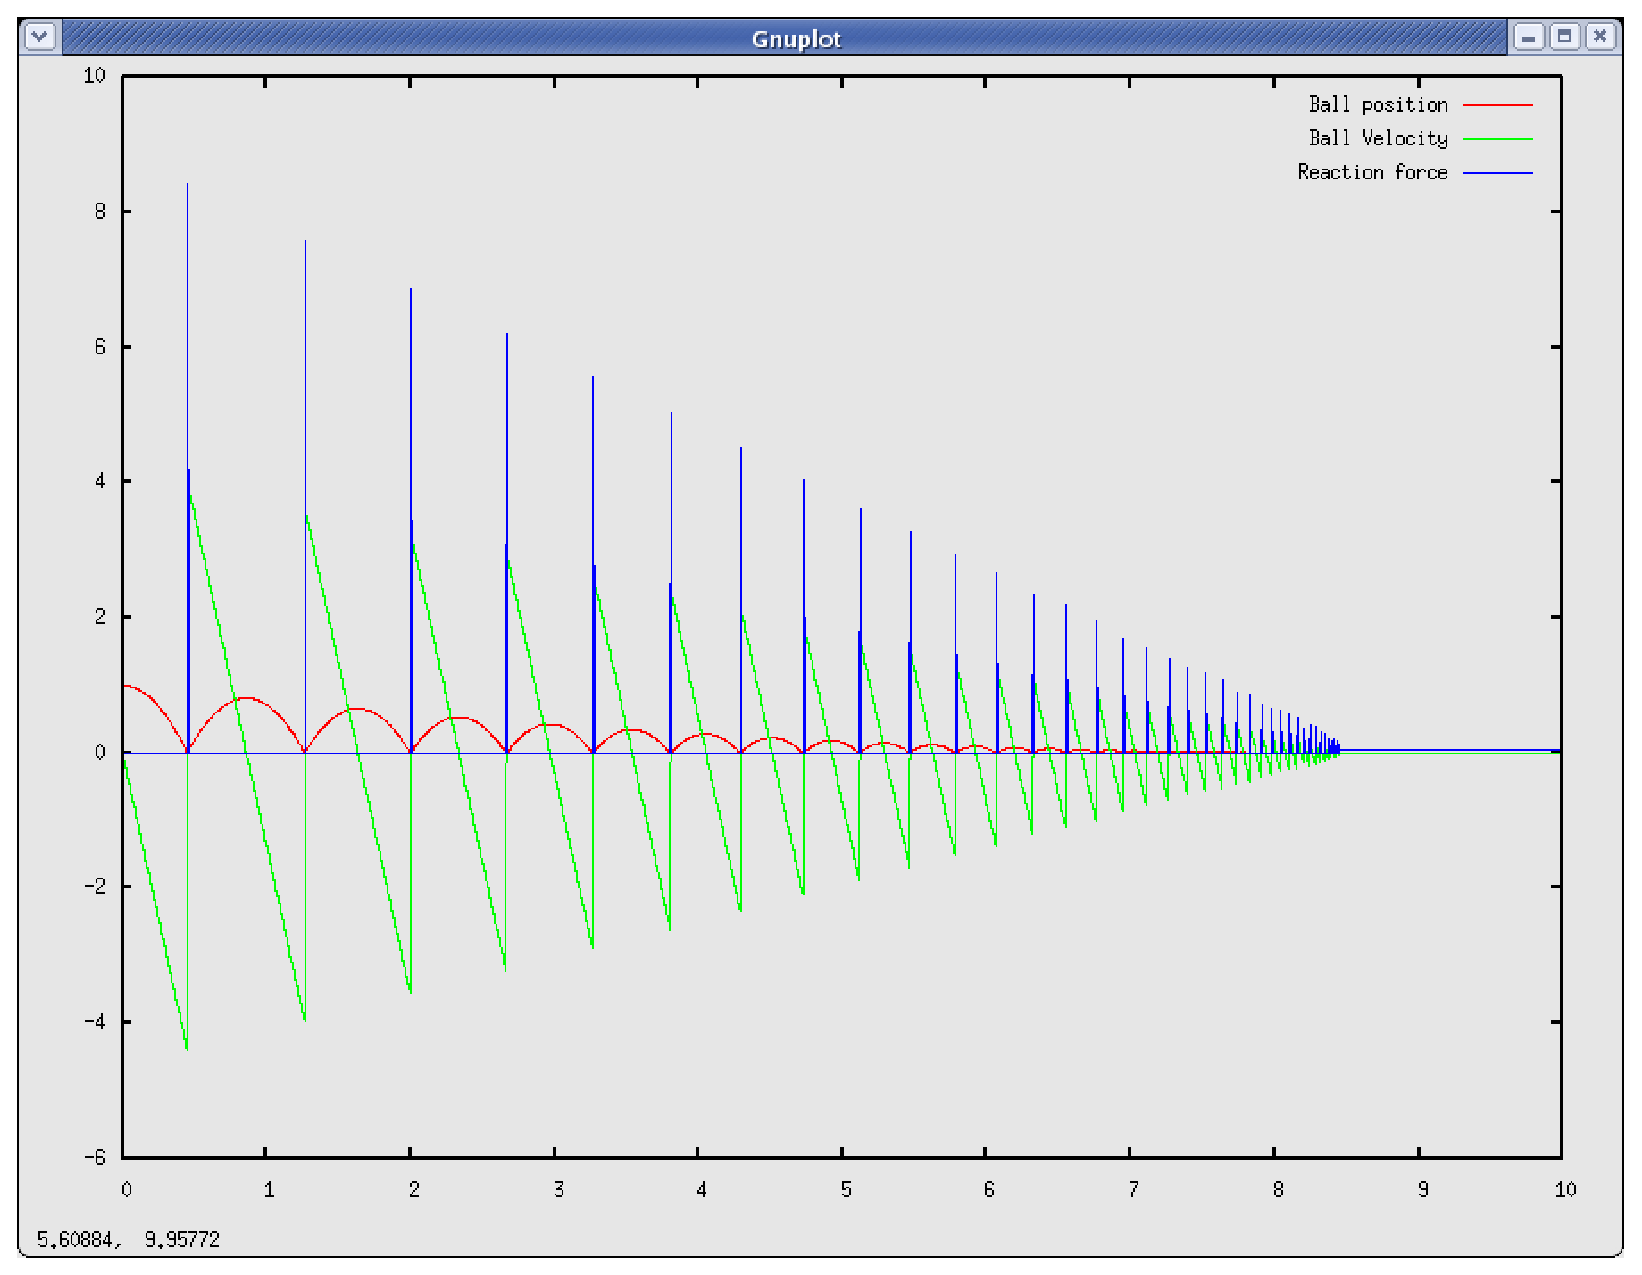
\includegraphics[scale=0.6, clip]{figure/BouncingBall.eps}
	\caption{Evolution of the BouncingBall in relation to the time}
	\label{fig: BouncingBall}
	\end{center}
	\end{figure}

\pagebreak

\section{RollingBalls}
\subsection{Purpose}
This sample has been made to test a non smooth dynamical system with several dynamical systems.\\
There are 3 moving points.\\
All the movements are only on 1 axis!\\
The 3 points are aligned. Each point is moving with different speeds, and will enter in contact with the other points during the simulation.

\subsection{Results}
We can see on the figure (\ref{fig: RollingBalls}) the position of the points and the speed of these points.\\

	\begin{figure}
	\begin{center}
	\includegraphics[scale=0.6, clip]{figure/RollingBalls.eps}
	\caption{Evolution of the RollingBalls in relation to the time}
	\label{fig: RollingBalls}
	\end{center}
	\end{figure}

\pagebreak

\section{DoubleContact}
\subsection{Purpose}
This sample has been made to test multiple contacts between dynamical systems.\\
There are 3 points of which 1 is static, and the 2 others are moving.\\
All the movement are only on 1 axis!\\
The 3 points are aligned. The 2 points that are moving are converging, and the convergence point correponds to the place of the third point.\\
Interactions are defined between points 1 and 2, 2 and 3, 1 and 3. So we have one contact point where the 3 interactions are activated.

\subsection{Results}
We can see on the figure (\ref{fig: DoubleContact}) the position of the points and the speed of these points.\\
When the contact occurs, the moving points are bouncing, changing there direction and losing some speed because of the Newton impact law coefficient (0.9). The middle point don't move because the 2 moving balls hit it with the same speed at the same time.
	\begin{figure}
	\begin{center}
	\includegraphics[scale=0.6, clip]{figure/DoubleContact.eps}
	\caption{Evolution of the DoubleContact balls in relation to the time}
	\label{fig: DoubleContact}
	\end{center}
	\end{figure}

\pagebreak

\section{Ball2D}
\subsection{Purpose}
This sample is the same as the BouncingBall, but this time, the point is moving in 2 dimensions.\\
The point is falling because of gravity force, has an advance velocity, and rebounds on a solid floor.\\

\subsection{Results}
We can see on the figure (\ref{fig: Ball2D}) the height of the point (Y axis) according to his position on the X axis.
	\begin{figure}
	\begin{center}
	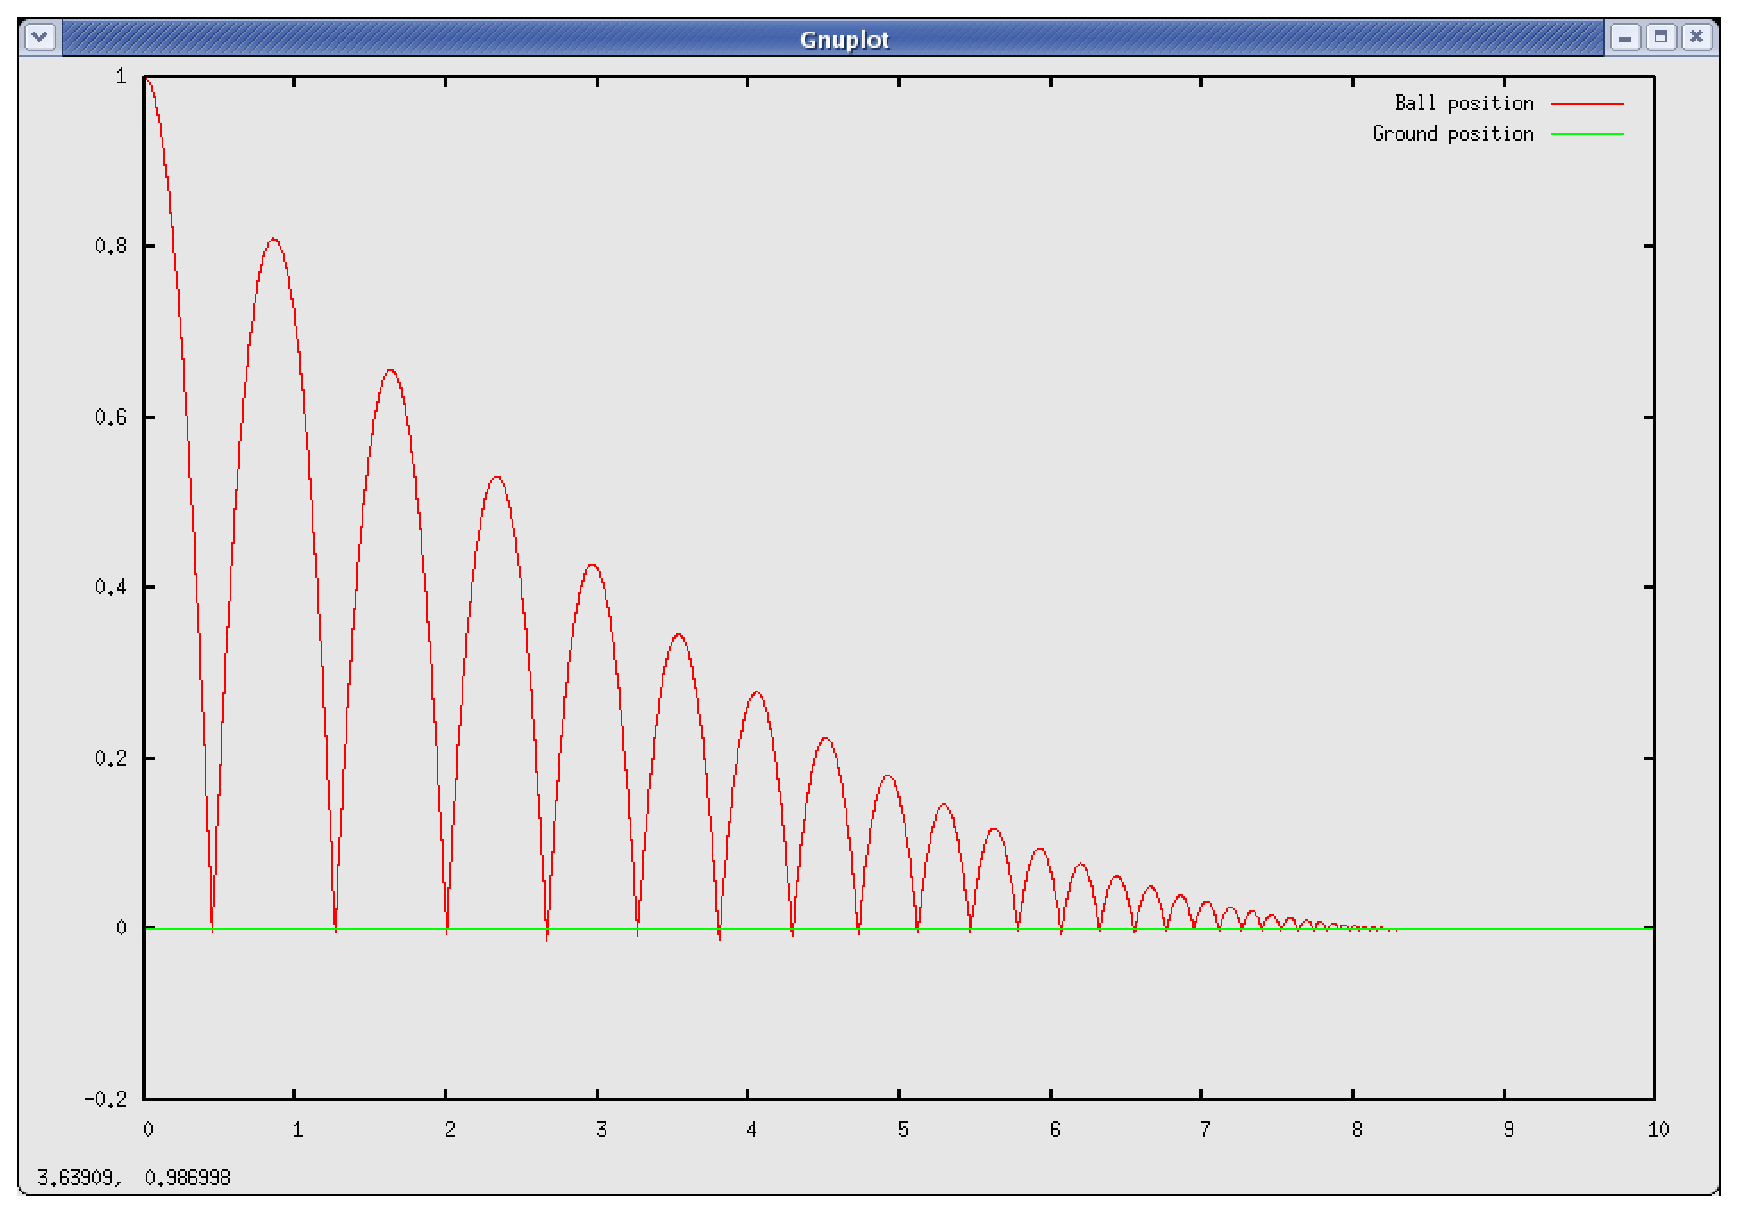
\includegraphics[scale=0.6, clip]{figure/Ball2D.eps}
	\caption{Evolution of the position of a BouncingBall in 2D}
	\label{fig: Ball2D}
	\end{center}
	\end{figure}

\pagebreak

%\section{UltraBalls}
% not yet functionnal

%---------------------------------------------------------------------%


%---------------------------------------------------------------------%
%\chapter{Reference}
%\label{Sec:UM-Reference}
%Reference

%---------------------------------------------------------------------%

\appendix
%---------------------------------------------------------------------%
\chapter{XML file sample}
\label{Sec:UM-XMLFile}
\begin{verbatim}

<SiconosModel Author="jbarbier">

	<Time>
		<t0>0</t0>
		<T>1000</T>
	</Time>

	<NSDS bvp='true'>
		<!-- DSs defined in the problem -->
		<DS_Definition>
			<LagrangianNLDS number='1'>
				<Id> toto </Id>
				<x vectorSize='6'>
					4.5454 454.5 5 5 5
					4.95222
				</x>
				
				<xDot vectorSize='6'>
					4.5454 454.5 8 8 8
					4.95222
				</xDot>

				<xMemory sizeMax='5'>				
				  <Memory vectorFile='./sample/vector.dat'/>
				  <Memory vectorSize='2'>
				  	54.54 5454212.5445456456
				  </Memory>
				  <Memory vectorFile='./sample/vector.dat'/>				  				  
				</xMemory>
				  
				<xDotMemory sizeMax='4'>
				  <Memory vectorFile='./sample/vector.dat'/>
				  <Memory vectorSize='2'>
				  	54.54 5454212.5445456456
				  </Memory>
				  <Memory vectorFile='./sample/vector.dat'/>				  				  
				</xDotMemory>
				
				<x0 vectorFile='./sample/vector2.dat'/>
				<StepsInMemory>8</StepsInMemory>
				
				<QNLInertia vectorPlugin="BasicPlugin:computeQNLInertia"/>
				<q vectorFile='./sample/vector.dat'/>
				<q0 vectorFile='./sample/vector.dat'/>
			
				<qMemory sizeMax='4'>
				  <Memory vectorFile='./sample/vector.dat'/>
				  <Memory vectorSize='2'>
				  	54.54 5454212.5445456456
				  </Memory>
				  <Memory vectorFile='./sample/vector.dat'/>				  				  
				</qMemory>								
				
				<Velocity vectorFile='./sample/vector.dat'/>
				<Velocity0 vectorFile='./sample/vector.dat'/>
				<VelocityMemory sizeMax='1'>
					<Memory vectorFile='./sample/vector.dat'/>
				</VelocityMemory>

				<Fint vectorPlugin="BasicPlugin:computeFInt"/>
				<Fext vectorPlugin="BasicPlugin:computeFExt"/>

				<JacobianQFint matrixPlugin="BasicPlugin:computeJacobianQFInt"/>
				<JacobianVelocityFint matrixPlugin="BasicPlugin:computeJacobianVelocityFInt"/>
 				<JacobianQQNLInertia matrixPlugin="BasicPlugin:computeJacobianQQNLInertia"/>
 				<JacobianVelocityQNLInertia matrixPlugin="BasicPlugin:computeJacobianVelocityQNLInertia"/>					  

				<ndof>3</ndof>
			
				<!-- Optional : if NSDS is bvp -->				
				<BoundaryCondition type="NLinear">					
				</BoundaryCondition>
			</LagrangianNLDS>
			
			<LagrangianTIDS number='2'>
				<!-- Commun at all DS -->
				<Id> toto </Id>
				<xDot vectorFile='./sample/vector2.dat'/>				

				<xMemory sizeMax='4'>				
				  <Memory vectorFile='./sample/vector2.dat'/>
				  <Memory vectorSize='2'>
				  	54.54 5454212.5445456456
				  </Memory>
				  <Memory vectorFile='./sample/vector2.dat'/>				  				  
				</xMemory>
				  
				<xDotMemory sizeMax='4'>
				  <Memory vectorFile='./sample/vector2.dat'/>
				  <Memory vectorSize="2">
				  	54.54 5454212.5445456456
				  </Memory>
				  <Memory vectorFile='./sample/vector2.dat'/>				  				  
				</xDotMemory>

				<x0 vectorFile='./sample/vector2.dat'/>
				<StepsInMemory>8</StepsInMemory>				
				
				<!-- Specific to LagrangianTIDS-->
				
				<q vectorFile='./sample/vector.dat'/>
				<q0 vectorFile='./sample/vector.dat'/>

				<qMemory sizeMax='4'>
				  <Memory vectorFile='./sample/vector.dat'/>
				  <Memory vectorSize='2'>
				  	54.54 5454212.5445456456
				  </Memory>
				  <Memory vectorFile='./sample/vector.dat'/>				  				  
				</qMemory>								
				
				<Velocity vectorFile='./sample/vector.dat'/>
				<Velocity0 vectorFile='./sample/vector.dat'/>
				<VelocityMemory sizeMax='1'>
					<Memory vectorFile='./sample/vector.dat'/>
				</VelocityMemory>

				<M matrixFile='./sample/matrix.dat'/>				
				
				<ndof>3</ndof>
				
				<K matrixFile='./sample/matrix.dat'/>
				<C matrixFile='./sample/matrix.dat'/>			

				<!-- Optional : if NSDS is bvp -->
				<BoundaryCondition type="Linear">
					<Omega vectorFile='./sample/vector.dat'/>
					<Omega0 matrixFile='./sample/matrix.dat'/>
					<OmegaT matrixFile='./sample/matrix.dat'/>				
				</BoundaryCondition>
			</LagrangianTIDS>		

			<LinearSystemDS number='3'>
				<!-- Commun at all DS -->
				<Id> tutu </Id>
				<n> 3 </n>
				<x vectorFile='./sample/vector.dat'/>
				
				<xDot vectorFile='./sample/vector.dat'/>				
				
				<xMemory sizeMax='4'>				
				  <Memory vectorFile='./sample/vector.dat'/>
				  <Memory vectorSize="2">
				  	54.54 5454212.5445456456
				  </Memory>
				  <Memory vectorFile='./sample/vector.dat'/>				  				  
				</xMemory>
				  
				<xDotMemory sizeMax='4'>
				  <Memory vectorFile='./sample/vector.dat'/>
				  <Memory vectorSize="2">
				  	54.54 5454212.5445456456
				  </Memory>
				  <Memory vectorFile='./sample/vector.dat'/>				  				  
				</xDotMemory>

				<x0 vectorFile='./sample/vector.dat'/>
				
				<StepsInMemory>8</StepsInMemory>				
				
				<!-- Specific to LinearSystemDS-->
				<A matrixFile='./sample/matrix.dat'/>
				<B matrixFile='./sample/matrix.dat'/>
				
				<u vectorFile='./sample/vector.dat'/>								
				<f vectorPlugin="BasicPlugin:computeF"/>
				
				<!-- Optional : if NSDS is bvp -->
				<BoundaryCondition type="Periodic">				
				</BoundaryCondition>
			</LinearSystemDS>

			
		</DS_Definition>

		<!-- Interactions defined in the problem -->		
		<Interaction_Definition>
			<Interaction number='1'>
				
				<Status>1</Status>
				<Id>totu</Id>
				<nInter>1</nInter>
				<!-- List of couple of DS concerned by this interaction -->			

				<DS_Concerned size='2'>
					<DS number='1' interactsWithDS_Number='2'/>			
					<DS number='1' interactsWithDS_Number='3'/>
				</DS_Concerned>					
											
				<!-- Relation of this interaction -->				
				<Interaction_Content>
					<LTI>
						<C matrixFile='./sample/matrix.dat'/>
						<D matrixFile='./sample/matrix.dat'/>
						<E matrixFile='./sample/matrix.dat'/>
						<a vectorFile='./sample/vector.dat'/>
					</LTI>			
	
					<!-- NS Law of this interaction -->				
					<ComplementarityCondition>
					</ComplementarityCondition>
				</Interaction_Content>
					
			</Interaction>
			
			<!-- A definition of a DS interaction, and list of couple of DSs who are concerned by it -->			
			<Interaction number='2'>

				<Status>1</Status>
				<Id>twtu</Id>
				<nInter>1</nInter>
				<!-- List of couple of DS concerned by this interaction -->			
				<DS_Concerned size='2'>
					<DS number='1' interactsWithDS_Number='2'/>		
					<DS number='1' interactsWithDS_Number='3'/>				
				</DS_Concerned>					
			
				<Interaction_Content>
					<!-- RELATION of this interaction -->				
					<LL>
						<H matrixFile='./sample/matrix.dat'/>
						<b vectorFile='./sample/vector.dat'/>
					</LL>							
	
					<!-- NS Law of this interaction -->				
					<Relay>
						<c>5.021</c>
						<d>5456.65</d>					
					</Relay>
				</Interaction_Content>
					
			</Interaction>							
				

			<!-- A definition of a DS interaction, and list of couple of DSs who are concerned by it -->			
			<Interaction number='3'>

				<Status>5 8</Status>
				<Id>tuto</Id>
				<nInter>1</nInter>
				<!-- List of couple of DS concerned by this interaction -->			
				<DS_Concerned size='2'>				
					<DS number='1' interactsWithDS_Number='2'/>		
					<DS number='1' interactsWithDS_Number='3'/>				
				</DS_Concerned>
			
				<Interaction_Content>
					<!-- Relation of this interaction -->				
					<LNL>
							<computeInput plugin="BasicPlugin:computeInput"/>
							<computeOutput plugin="BasicPlugin:computeOutput"/>
					</LNL>
	
					<!-- NS Law of this interaction -->				
					<NewtonImpactLaw>
						<e>0.95</e>				
					</NewtonImpactLaw>
				</Interaction_Content>
		                
					
			</Interaction>							
		</Interaction_Definition>
	</NSDS>
	
	<!-- Strategy to use in order to solve the problem -->				
	<Strategy type='TimeStepping'>
		<TimeDiscretisation isConstant='true'>	
			<h>0.65</h>
			<N>52</N>
			<tk vectorSize='2'>5.545 548.2</tk>
			<hMin>54.534</hMin>
			<hMax>105.54</hMax>
		</TimeDiscretisation>				

		<!-- One Step Integrators -->				
		<OneStepIntegrator_Definition>
			<Moreau>
				<DS_Concerned size='1'>
					<DS number='2'/>			
				</DS_Concerned>
				<r>4</r>
				<Theta> 0.5</Theta>
				<W matrixColSize="0" matrixRowSize="0"/>
			</Moreau>					

			<!-- A definition of a OneStepIntegrator, and list of couple of DSs who are concerned by it -->					
			<Adams>
				<DS_Concerned size='1'>								
					<DS number='1'/>
				</DS_Concerned>
				<r>4</r>
			</Adams>
					
			<!-- A definition of a OneStepIntegrator, and list of couple of DSs who are concerned by it -->										
			<LSODAR>
				<DS_Concerned size='1'>
					<DS number='3'/>
				</DS_Concerned>
				<r>4</r>
			</LSODAR>
		</OneStepIntegrator_Definition>

	 	<LCP>
			<!-- General for one step NS problem -->					
			<n>8</n>			
					
			<!-- Specific at LCP -->						
			<M matrixFile='./sample/matrix.dat'/>
			<q vectorFile='./sample/vector.dat'/>
			
			<Interaction_Concerned size='3'>												
				<Interaction number='1'/>
				<Interaction number='2'/>
				<Interaction number='3'/>
			</Interaction_Concerned>			
			
	 	</LCP>		
	</Strategy>	
</SiconosModel>
\end{verbatim}

%---------------------------------------------------------------------%
\chapter{High level commands}
\label{Sec:UM-Command}
% \verbatiminput{BouncingBall.cpp}

These functions are the highest level of granularity of command to drive a simulation with the platform :

\begin{itemize}
\item\textbf{LoadXMLFile([file name])}
  Allows to load a SICONOS XML file. [file name] is an absolute path (tbc).  

\item \textbf{InitStrategy()}
  Initializes the strategy of simulation.

\item \textbf{GetStartTime()}
  Gets the starting time of simulation.

\item  \textbf{GetCurrentTime(})
  Gets the current time of simulation.

\item \textbf{GetEndTime()}
  Gets the final time of simulation.

\item\textbf{ NextStep()}
  Passes to next step of simulation, and saves values in memory if needed.

\item \textbf{ComputeFreeState()}
  Computes new state of the system without applying constraints

\item \textbf{FormaliseOneStepNSProblem()}
  Formalizes non-smooth problem.

\item \textbf{ComputeOneStepNSProblem()}
  Computes one step of the problem.

\item \textbf{UpdateState()}
  Updates state of the system regards to result of computing problem (active relations, etc.).

\item \textbf{SaveXMLFile([file name])}
  Saves the state of the system in a SICONOS XML file.

\end{itemize}

%---------------------------------------------------------------------%



\printglosstex(acr)[p]


\listoffigures
\listoftables
\cleardoublepage
\bibliographystyle{plainnat}
\bibliography{./Biblio/String,./Biblio/Cp.bib,./Biblio/Optim.bib,./Biblio/Contact.bib,./Biblio/NonSmooth.bib,./Biblio/Leger.bib,./Biblio/Petri.bib}

\end{document} 
